\chapter{奇异关联子与全息张量网络}
\label{chap:strange-correlator}

在前两章中,我们分别介绍了拓扑序和张量网络的基本概念。作为二维拓扑序的重要模型,弦网模型的 Hamilton 量可以表示为一系列局域算符之和,因此用张量网络来表示其基态也成为了一种很自然的想法。而将弦网模型的基态波函数与某些特定的直积态做内积,可以直接得到相应临界格点模型的配分函数。这种称为\emph{奇异关联子} (strange correlator) 的构造,不仅使我们能够计算相应 CFT 的中心荷和能谱,还给出了一种重整化算符的构造方案,进而使我们得以将体 (bulk) 和边界 (boundary) 联系在一起,并以此来构建全息张量网络 (holographic tensor network)。

\section{弦网模型基态的张量网络表示}

\subsection{四面体对称性}
\label{subsec:tetrahedral-symmetry}

为了叙述与计算的方便,我们先来澄清一下 $F$ 符号的定义,并介绍其对称性。在式~\eqref{eq:f-move} 和 \eqref{eq:string-net-local-rules} 中分别给出了 $F$ 符号的两种定义:
\begin{equation}
  \begin{aligned}
       \tikzinput{category/f-symbol-1}
    &= \sum_y \, \bigl[ F^{abc}_d \bigr]_{xy} \tikzinput{category/f-symbol-2}, \\
       \tikzinput{category/f-symbol-3}
    &= \sum_m F^{ijm}_{kln} \tikzinput{category/f-symbol-4}.
  \end{aligned}
\end{equation}
容易知道 $[F^{ijk}_l]_{xy}=F^{jix}_{lky}$。在本文中我们主要使用第一种定义。另一方面,根据式~\eqref{eq:f-move},我们有
\begin{equation}
    \bigl[ F^{abc}_d \bigr]_{xy}
  = \frac{\tr \, \Biggl[
      \Biggl( \tikzinput{category/f-symbol-small-2} \Biggr)^\dagger \,
      \tikzinput{category/f-symbol-small-1}
    \Biggr]}{\tr \, \Biggl[
      \Biggl( \tikzinput{category/f-symbol-small-2} \Biggr)^\dagger \,
      \tikzinput{category/f-symbol-small-2}
    \Biggr]}
  = \frac{\tikzinput{category/f-symbol-trace-1}}{\tikzinput{category/f-symbol-trace-2}}.
\end{equation}
这里分母部分可以利用环路消除 \eqref{eq:loop-removal} 式化简:
\begin{equation}
  \tikzinput{category/f-symbol-trace-2} = \sqrt{d_a d_b d_c d_d},
\end{equation}
而分子部分则等价于一个正四面体,于是
\begin{equation}
    \bigl[ F^{abc}_d \bigr]_{xy}
  = \sqrt{d_x d_y} \, \begin{bmatrix} a & b & x \\ c & d & y \end{bmatrix}
  = \frac{1}{\sqrt{d_a d_b d_c d_d}} \, \Tetrahedron xbdyca.
  \label{eq:tetrahedra-symbol}
\end{equation}
式中
\begin{equation}
    \begin{bmatrix} a & b & c \\ i & j & k \end{bmatrix}
  = \frac{1}{\sqrt{d_a d_b d_c d_i d_j d_k}} \, \Tetrahedron cbjkia
\end{equation}
称为\emph{四面体符号} (tetrahedral symbol) 或 \emph{$6j$ 符号} ($6j$-symbol),它的对称性(以及相应 $F$ 符号的对称性)可以从四面体的几何性质中获得:
\begin{align}
     \begin{bmatrix} a & b & c \\ i & j & k \end{bmatrix}
  &= \begin{bmatrix} b & c & a \\ j & k & i \end{bmatrix}
   = \begin{bmatrix} c & a & b \\ k & i & j \end{bmatrix}, \\
     \begin{bmatrix} a & b & c \\ i & j & k \end{bmatrix}
  &= \begin{bmatrix} a & c & b \\ i & k & j \end{bmatrix}
   = \begin{bmatrix} c & b & a \\ k & j & i \end{bmatrix}
   = \begin{bmatrix} b & a & c \\ j & i & k \end{bmatrix}, \\
     \begin{bmatrix} a & b & c \\ i & j & k \end{bmatrix}
  &= \begin{bmatrix} a & j & k \\ i & b & c \end{bmatrix}
   = \begin{bmatrix} i & b & k \\ a & j & c \end{bmatrix}
   = \begin{bmatrix} i & j & c \\ a & b & k \end{bmatrix}.
\end{align}
以上三组等式分别对应了四面体对称群 $A_4$ 中绕顶角的旋转(列轮换)、镜像(交换两列)和绕对边连线的旋转(交换两行的部分)。注意整行的交换一般来说并不相等。这一性质为\emph{四面体对称性} (tetrahedral symmetry)\cite{aasen2020topological,fuchs2023tetrahedral}。利用 $F$ 移动和环路消除,还可以得到下面的关系式:
\begin{equation}
    \tikzinput{string-net/vertex-2}
  = \sqrt{d_\alpha d_\beta d_\gamma} \, \begin{bmatrix} a & b & c \\ \alpha & \beta & \gamma \end{bmatrix} \Vertex kij
  = \frac{1}{\sqrt{d_i d_j d_k}} \, \Tetrahedron ik\gamma\alpha\beta j \Vertex kij,
\end{equation}
这也被称为\emph{星—三角变换} (star-triangle transformation)。

\subsection{弦网模型的基态}
\label{subsec:string-net-ground-state}

接下来我们来给出弦网模型基态的张量网络表示\cite{gu2009tensor2,buerschaper2009explicit}。由于弦网模型的 Hamilton 量
\begin{equation}
  H = -\sum_v A_v - \sum_p B_p
\end{equation}
是严格可解的,即 $H$ 可以表示成一系列相互对易的投影算符之和,因而它的基态可以通过这些投影算符的本征子空间给出。式中,电荷算符 $A_v$ 指定了每个顶点处的融合规则,磁通算符 $B_p$ 是 $B_p^s$ 按量子维数的线性组合,而 $B_p^s$ 则可以图形化地视为能在方块 $p$ 处生成一个孤立环路的算符(具体定义见 \ref{subsec:string-net-hamiltonian} 小节)。

弦网模型的基态波函数 $\ket{\psi_0}$ 可以通过在真空态 $\ket{\varnothing}$ 上作用全部的 $B_p$ 算符得到。如上所言,每个 $B_p$ 算符都是一个方块内部由对象 $R$ 构成的环路,而
\begin{equation}
  \tikzinput{string-net/string-1}
  \enspace = \sum_i \frac{d_i}{D^2}
  \tikzinput{string-net/string-2}
\end{equation}
则是任意子按量子维数的加权叠加。因此有
\begin{equation}
    \ket{\psi_0} = \prod_p B_p \ket{\varnothing}
  = \prod_p B_p \, \ket[\Bigg]{\, \tikzinput{string-net/loop-1} \,}
  = \ket[\Bigg]{\, \tikzinput{string-net/loop-2} \,}.
\end{equation}

为了给出 $\ket{\psi_0}$ 一种\emph{对称化}的张量网络表示,我们必须从一开始就同等对待六边形的每个边以保持对称性。需要指出的是,文献 \parencite{buerschaper2009explicit} 中通过引入奇偶子网格来构造张量网络的手段不能很好地保留旋转对称性。这里,我们需将权重(量子维数)$d_i$ 平均分配到 $R$ 环路的六个边上,使得它们在互相连接时也有良好定义:
\begin{equation}
  \begin{aligned}
       \VirutalHexagon{\draw [very thick, draw=MaterialRed] (-30:0.8) -- (30:0.8)} \enspace
    &= \sum_i \left( \frac{d_i}{D^2} \right)^{1/6} \enspace
       \VirutalHexagon{\draw [thick] (-30:0.8) node [left] {$i$} -- (30:0.8)} \, , \\
       \VirutalHexagon{\draw [very thick, draw=MaterialRed] (-30:0.8) -- (30:0.8) -- (90:0.8)} \enspace
    &= \sum_i \left( \frac{d_i}{D^2} \right)^{1/3} \enspace
       \VirutalHexagon{\draw [thick] (-30:0.8) node [left] {$i$} -- (30:0.8) -- (90:0.8)} \, , \\
       \VirutalHexagon{\draw [very thick, draw=MaterialRed] (0,0) circle [radius=0.7]} \enspace
    &= \sum_i \frac{d_i}{D^2} \enspace
       \VirutalHexagon{\draw [thick] (0,0) circle [radius=0.7] node [right=-0.2em] {$i$}} \, .
  \end{aligned}
\end{equation}
对于邻接的六边形,我们可以在两个相邻的 $R$ 环路间执行 $F$ 移动:
\begin{align}
     \tikzinput{string-net/adjacent-loop-1} \enspace
  &= \sum_{i,j} \biggl( \frac{d_i d_j}{D^4} \biggr)^{1/6} \enspace
     \tikzinput{string-net/adjacent-loop-2} \notag \\
  &= \sum_{i,j} \biggl( \frac{d_i d_j}{D^4} \biggr)^{1/6} \sum_k \sqrt{\frac{d_k}{d_i d_j}} \enspace
     \tikzinput{string-net/f-move-1} \notag \\
  &= \sum_{i,j,k} \bigl( D^2 d_i d_j \bigr)^{-1/6} d_k^{1/4} \cdot \bigl( D^2 d_i d_j \bigr)^{-1/6} d_k^{1/4} \enspace
     \tikzinput{string-net/f-move-1} \,
   = \tikzinput{string-net/f-move-2} \, .
\end{align}
式中,蓝线和紫线表示各任意子按照对应量子维数的加权叠加,并且分别带有 $(D^2 d_i d_j)^{-1/6}$ 和 $d_k^{1/4}$ 的因子。在对所有的 $R$ 环路执行 $F$ 移动之后,$\ket{\psi_0}$ 现在可以表示为
\begin{equation}
  \ket{\psi_0} = \ket[\Bigg]{\, \tikzinput{string-net/vertices}}.
\end{equation}
它可以通过对位于顶点处的局域构建块进行缩并得到,而这些构建块可以用任意子基 (anyon basis) 表示为
\begin{align}
     \tikzinput{string-net/vertex-1} \enspace
  &= \sum_{i,j,k} \sum_{\alpha,\beta,\gamma} D^{-1} (d_i d_j d_k)^{1/4} (d_\alpha d_\beta d_\gamma)^{-1/3} \,
     \tikzinput{string-net/vertex-2} \notag \\
  &= \sum_{i,j,k} \sum_{\alpha,\beta,\gamma} D^{-1} (d_i d_j d_k)^{-1/4} (d_\alpha d_\beta d_\gamma)^{-1/3}
     \Tetrahedron ik\gamma\alpha\beta j \Vertex kij.
\end{align}
这样我们就获得了六边形网格中三角形张量的对称形式:
\begin{align}
  \Triangle jki\alpha\beta\gamma
  &= D^{-1} (d_i d_j d_k)^{-1/4} (d_\alpha d_\beta d_\gamma)^{-1/3} \,
    \Tetrahedron ik\gamma\alpha\beta j \notag \\
  &= D^{-1} (d_\alpha d_\beta d_\gamma)^{1/6} (d_i d_j d_k)^{-1/4} (d_\alpha d_\beta d_\gamma)^{-1/2} \,
    \Tetrahedron ik\gamma\alpha\beta j.
  \label{eq:unit-of-string-net-honeycomb}
\end{align}
对于更一般的情形,因子 $1/6$ 需要根据闭合环路中每条边的贡献进行修正。在任意三价图(每个顶点与三条边相连)中,归一化的三角形张量可以写成
\begin{align}
  \Triangle jki\alpha\beta\gamma
  &= D^{-2 (1/n_\alpha + 1/n_\beta + 1/n_\gamma)}
    \bigl( d_\alpha^{1/n_\alpha} d_\beta^{1/n_\beta} d_\gamma^{1/n_\gamma} \bigr) \notag \\
  &\qquad \cdot (d_i d_j d_k)^{-\frac14} (d_\alpha d_\beta d_\gamma)^{-\frac12} \,
    \Tetrahedron ik\gamma\alpha\beta j,
  \label{eq:unit-of-string-net-general}
\end{align}
这些三角形张量每条边带有三个指标,外面的两个是\emph{虚拟指标}或\emph{辅助指标},它们会在平面内互相缩并掉;中间的一个则是\emph{物理指标},它们会伸出平面外,并且不会被缩并掉。可以看出,这实际上也是一种 PEPS 张量网络(见 \ref{subsec:mps-generalization} 小节)。

\begin{figure}[htb]
  \centering
  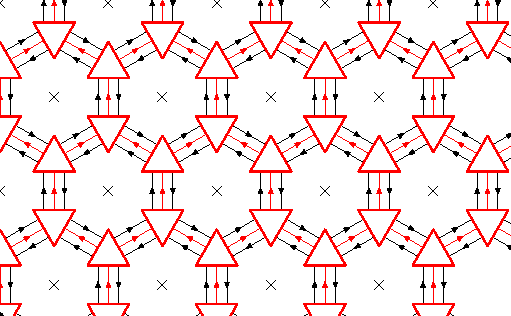
\includegraphics[width=0.6\textwidth]{images/string-net-peps.pdf}
  \caption[弦网模型基态的 PEPS 张量网络表示]{弦网模型基态的 PEPS 张量网络表示。图片来源:\parencite{buerschaper2009explicit}。}
  \label{fig:string-net-peps}
\end{figure}

\section{奇异关联子}
\label{sec:strange-correlator}

\emph{奇异关联子} (strange correlator) 最早用来在对称保护拓扑序 (symmetry protected topological order, SPT)\footnote{尽管名称中带有“拓扑序”,但 SPT 态中只有短程纠缠,这与本文所说的拓扑序(具有长程纠缠,见 \ref{sec:topological-order} 节)实际上是不同的。} 中寻找不同的相\cite{you2014wave},之后则被推广到了弦网模型中\cite{vanhove2018mapping,lootens2019cardy,vanhove2022topological}。通过将 2+1 维弦网模型的 PEPS 基态波函数 $\ket{\Psi_\text{SN}}$ 与某些特定的直积态 $\bra{\Omega}$ 做内积,可以获得二维临界格点模型的配分函数
\begin{equation}
  Z = \langle\Omega|\Psi_\text{SN}\rangle.
\end{equation}
在热力学极限下,配分函数 $Z$ 可由对应的共形场论 (CFT) 来描述。如图~\ref{fig:peps-strange-correlator} 所示,对于由三角形张量单元构成的 PEPS 张量网络,直积态 $\bra{\Omega}$ 相当于为其提供了特定的边界条件,即把物理指标固定到某些值上,而角落上的自由度则需求和。

\begin{figure}[htb]
  \centering
  \tikzinput{strange-correlator}
  \caption[奇异关联子的构造]{奇异关联子的构造。其中绿线表示投影到特定值(即与某直积态做内积)之后的物理指标,灰线表示需要求和的辅助指标。整个张量网络完全缩并后即为对应的配分函数。}
  \label{fig:peps-strange-correlator}
\end{figure}

\subsection{例子:Fibonacci 模型}
\label{subsec:strange-correlator-fib}

接下来,我们利用 \ref{subsec:fusion-category-examples} 小节中所给出的 Fibonacci 和 Ising 两种融合范畴的数据来构造相应的奇异关联子。Fibonacci 弦网模型定义在六边形网格上,它包含 $\1$ 和 $\tau$ 两种简单对象(任意子),量子维数分别为 $d_{\1}=1$、$d_\tau=\varphi$,其中 $\varphi=(1+\sqrt5)/2$ 是黄金比。融合规则为
\begin{equation}
  \1 \times \1 = \1, \quad
  \1 \times \tau = \tau \times \1 = \tau, \quad
  \tau \times \tau = \1 + \tau,
\end{equation}
$F$ 符号为
\begin{equation}
  [F^{\tau\tau\tau}_\tau]_{ij} = \dfrac1\varphi \begin{pmatrix} 1 & \sqrt\varphi \\ \sqrt\varphi & -1 \end{pmatrix}, \quad
  i,j \in \{\1, \tau\}.
\end{equation}
唯一非平凡的四面体以及对应的三角形张量为
\begin{equation}
  \begin{aligned}
       \Tetrahedron \tau mn\tau\tau\tau
    &= \sqrt{d_\tau d_\tau d_\tau d_\tau} \bigl[ F^{\tau\tau\tau}_\tau \bigr]_{mn}
     = \varphi^2 \bigl[ F^{\tau\tau\tau}_\tau \bigr]_{mn}, \\
       \Triangle \tau\tau mn\tau\tau
    &= (d_\tau d_\tau d_m)^{-\frac14} (d_\tau d_\tau d_n)^{-\frac13} \Tetrahedron \tau mn\tau\tau\tau \\
    &= \varphi^{\frac56} d_m^{-\frac14} d_n^{-\frac13} \bigl[ F^{\tau\tau\tau}_\tau \bigr]_{mn}, \enspace
       m,n \in \{\1,\tau\}.
  \end{aligned}
\end{equation}
在我们的奇异关联子构造中,所有的物理指标都会被选取为 $\tau$,因而这时将得到两种三角形张量单元:
\begin{equation}
    \Triangle \tau\tau\tau\tau\tau\tau
  = \varphi^{\frac14} \bigl[ F^{\tau\tau\tau}_\tau \bigr]_{\tau\tau} = -\varphi^{-\frac34}, \quad
    \Triangle \tau\tau\tau\1\tau\tau
  = \varphi^{\frac{7}{12}} \bigl[ F^{\tau\tau\tau}_\tau \bigr]_{\tau\1} = \varphi^{\frac{1}{12}}.
\end{equation}

\subsection{例子:Ising 模型}

为了与经典二维 Ising 模型相对应,我们考虑一个定义在正方形和八边形交错的网格上、由 $\1$、$\sigma$ 和 $\psi$ 三种简单对象构成的 Ising 弦网模型。各任意子对应的量子维数分别为 $d_{\1}=d_\psi=1$、$d_\sigma=\sqrt2$,融合规则为
\begin{equation}
  \begin{gathered}
  \1 \times \1 = \psi \times \psi = \1, \quad
  \1 \times \sigma = \sigma \times \1 = \sigma \times \psi = \psi \times \sigma = \sigma, \\
  \1 \times \psi = \psi \times \1 = \psi, \quad
  \sigma \times \sigma = \1 + \psi,
  \end{gathered}
\end{equation}
$F$ 符号为
\begin{equation}
  [F^{\psi\sigma\psi}_\sigma]_{\sigma\sigma} = [F^{\sigma\psi\sigma}_\psi]_{\sigma\sigma} = -1, \quad
  [F^{\sigma\sigma\sigma}_\sigma]_{ij} = -\dfrac{1}{\sqrt2} \begin{pmatrix} 1 & 1 \\ 1 & -1 \end{pmatrix}, \quad
  i,j \in \{\1, \psi\}.
\end{equation}
于是四面体和三角形张量为:
\begin{align}
     \Triangle \sigma\sigma\1\1\sigma\sigma
  &= (d_{\1} d_\sigma d_\sigma)  ^{-\frac14} (d_{\1} d_\sigma d_\sigma)  ^{-\frac13}
     \Tetrahedron \1\sigma\sigma\1\sigma\sigma
     = 2^{-\frac{1}{12}}, \notag \displaybreak[0] \\
     \Triangle \sigma\sigma\1\psi\sigma\sigma
  &= (d_{\1} d_\sigma d_\sigma)  ^{-\frac14} (d_\sigma d_\sigma d_\psi)^{-\frac13}
     \Tetrahedron \1\sigma\sigma\psi\sigma\sigma
     = 2^{-\frac{1}{12}}, \notag \displaybreak[0] \\
     \Triangle \sigma\sigma\psi\1\sigma\sigma
  &= (d_\sigma d_\sigma d_\psi)^{-\frac14} (d_{\1} d_\sigma d_\sigma)  ^{-\frac13}
     \Tetrahedron \psi\sigma\sigma\1\sigma\sigma
     = 2^{-\frac{1}{12}}, \notag \displaybreak[0] \\
     \Triangle \sigma\sigma\psi\psi\sigma\sigma
  &= (d_\sigma d_\sigma d_\psi)^{-\frac14} (d_\sigma d_\sigma d_\psi)^{-\frac13}
     \Tetrahedron \psi\sigma\sigma\psi\sigma\sigma
     = -2^{-\frac{1}{12}}.
\end{align}
在 Ising 模型的奇异关联子构造中,我们需要将物理指标投影到直积态
\begin{equation}
  \bra{\omega(\beta)} = \sqrt2 \, \bigl( \cosh\beta \bra{\1} + \sinh\beta \bra{\psi} \bigr)
\end{equation}
上面。为了得到正方形网格的结构,我们用 8 个三角形组成一个带有 4 个指标的八边形张量单元:
\begin{equation}
  A_{ijkl} = \tikzinput{ising/octagon} \quad \text{where} \quad
  i, j, k, l = \1 \text{ or } \psi, \quad
  \tikzinput{ising/line-sigma} \, = \sigma, \quad
  \tikzinput{ising/line-omega} \, = \omega.
  \label{eq:ising-octagon}
\end{equation}
注意此时物理指标已被求和,而辅助指标 $i$、$j$、$k$、$l$ 得以保留。为了得到 $A_{ijkl}$ 的值,我们先计算每一对三角形:
\begin{equation}
  \tikzinput{ising/triangles-1} = \tikzinput{ising/triangles-2} =
  \begin{cases}
    2^{\frac13} \bigl( \cosh\beta + \sinh\beta \bigr) = 2^{\frac13} \ee^\beta,
      & (i,j) = (\1,\1) \text{ or } (\psi, \psi); \\
    2^{\frac13} \bigl( \cosh\beta - \sinh\beta \bigr) = 2^{\frac13} \ee^{-\beta},
      & (i,j) = (\1,\psi) \text{ or } (\1, \psi).
  \end{cases}
\end{equation}
于是
\begin{equation}
  A_{\1\1\1\1} = A_{\psi\psi\psi\psi} = 2^{\frac43} \ee^{4\beta}, \quad
  A_{\1\psi\1\psi} = A_{\psi\1\psi\1} = 2^{\frac43} \ee^{-4\beta}, \quad
  \text{others} = 2^{\frac43}.
  \label{eq:ising-tensor-from-sc}
\end{equation}
这和围绕一个方块的 Ising 相互作用(4 个自旋)的张量表示 \eqref{eq:ising-tensor} 是一致的,只相差一个整体因子:
\begin{equation}
  A_{ijkl}
    := A_{\sigma_i \sigma_j \sigma_k \sigma_l}
    = \ee^{\beta(\sigma_i\sigma_j + \sigma_j\sigma_k + \sigma_k\sigma_l + \sigma_l\sigma_i)},
  \label{eq:ising-tensor}
\end{equation}

% TODO: dual lattice
把这些八边形张量移动 $1/2$ 格可以获得对偶网格的张量表示
\begin{equation}
  \tilde{A}_{ijkl} = \, \tikzinput{ising/dual-octagon} \quad \text{where} \quad
  i, j, k, l = \1 \text{ or } \psi.
\end{equation}
此时
\begin{equation}
  \tikzinput{ising/dual-triangles-1} = \tikzinput{ising/dual-triangles-2} =
  \begin{cases}
    2^{\frac13} \bigl( \cosh\beta + \sinh\beta \bigr) = 2^{\frac13} \ee^\beta,
      & (i,j) = (\1,\1) \text{ or } (\psi, \psi); \\
    2^{\frac13} \bigl( \cosh\beta - \sinh\beta \bigr) = 2^{\frac13} \ee^{-\beta},
      & (i,j) = (\1,\psi) \text{ or } (\1, \psi).
  \end{cases}
\end{equation}
利用 Kramers--Wannier 对偶,即令 $A=\tilde{A}$,就可以得到临界温度
\begin{equation}
  \ee^{2\beta_{\text{c}}} = \sqrt{2} + 1 \implies \beta_{\text{c}} = \frac12 \log(1 + \sqrt{2}).
\end{equation}

\subsection{中心荷的计算}
\label{subsec:central-charge}

得到奇异关联子后,我们可以用标准的张量网络方法对其进行分析。例如,我们可以利用在 \ref{subsec:mps-time-evolution} 小节中介绍的 iTEBD 算法来计算中心荷,其基本思路是:

\begin{enumerate}
  \item 利用奇异关联子构造正方形张量单元 $A_{ijkl}$。在 Ising 的情况中,我们已经得到了这样的表示[式~\eqref{eq:ising-octagon}];而对于 Fibonacci 模型,我们需要把两个三角张量形拼合成一个正方形:
    \begin{equation}
      A_{ijkl} = \tikzinput{fibonacci/square-1}.
    \end{equation}
  \item 按照 iTEBD 算法,用 $A_{ijkl}$ 作为 iMPO 对随机的初始态进行演化,得到正则化的不动点 iMPS $\{\Gamma,\lambda\}$。
  \item 注意 $\lambda$ 是一个对角矩阵,其对角元可用来计算关联长度 $\xi$ 和 von Neumann 纠缠熵 $S_A$:
    \begin{equation}
      \xi = -\frac{1}{\log|\lambda_2 / \lambda_1|}, \quad
      S_A = \sum_i \lambda_i^2 \log \lambda_i^2
    \end{equation}
  \item 利用关联长度与纠缠熵之间满足的关系式
    \begin{equation}
      S_A \sim \frac{c}{6} \log \xi,
    \end{equation}
    可以对使用不同的连接维数 $\chi$ 所获得的数据进行拟合,即可得到中心荷 $c$。
\end{enumerate}

我们使用连接维数 $\chi\in\{8,9,\dots,27\}$ 来进行计算,拟合结果如图~\ref{fig:central-charge} 所示。得到的中心荷为
\begin{equation}
  c_{\text{Ising}} \simeq 0.499 \pm 0.004, \quad
  c_{\text{Fib}}   \simeq 0.792 \pm 0.004.
\end{equation}
这与对应 CFT 给出的理论值 $1/2$ 和 $4/5$ 是非常接近的,说明通过奇异关联子的确可以从弦网模型基态波函数出发得到正确的 CFT 不动点张量。

\begin{figure}[htb]
  % TODO: update image
  \centering
  \subcaptionbox{Ising 模型}{%
    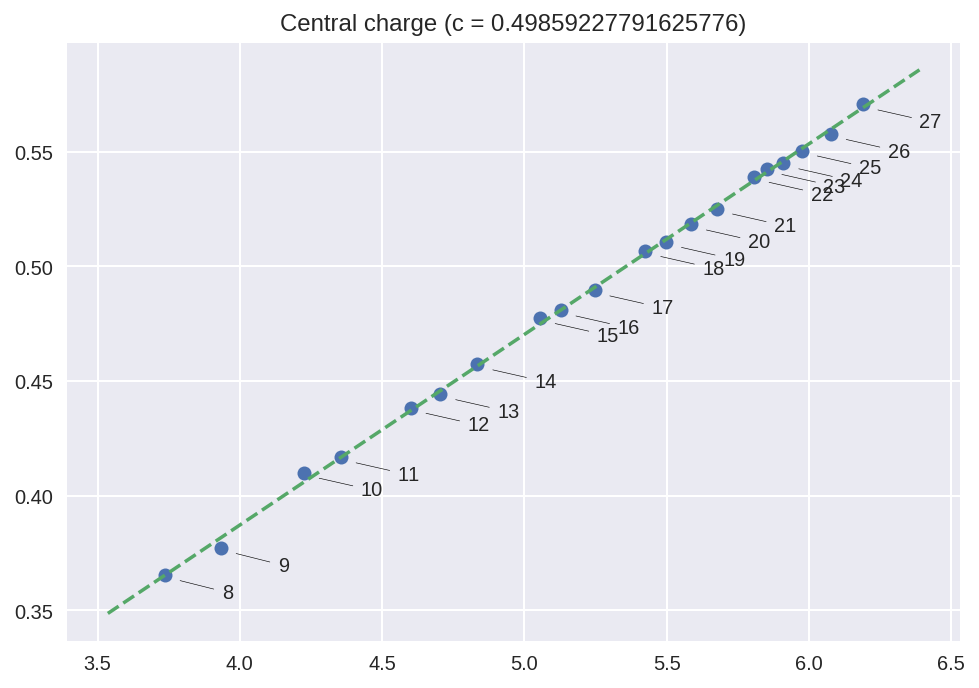
\includegraphics[width=0.45\textwidth]{images/ising-central-charge.png}} \quad
  \subcaptionbox{Fibonacci 模型}{%
    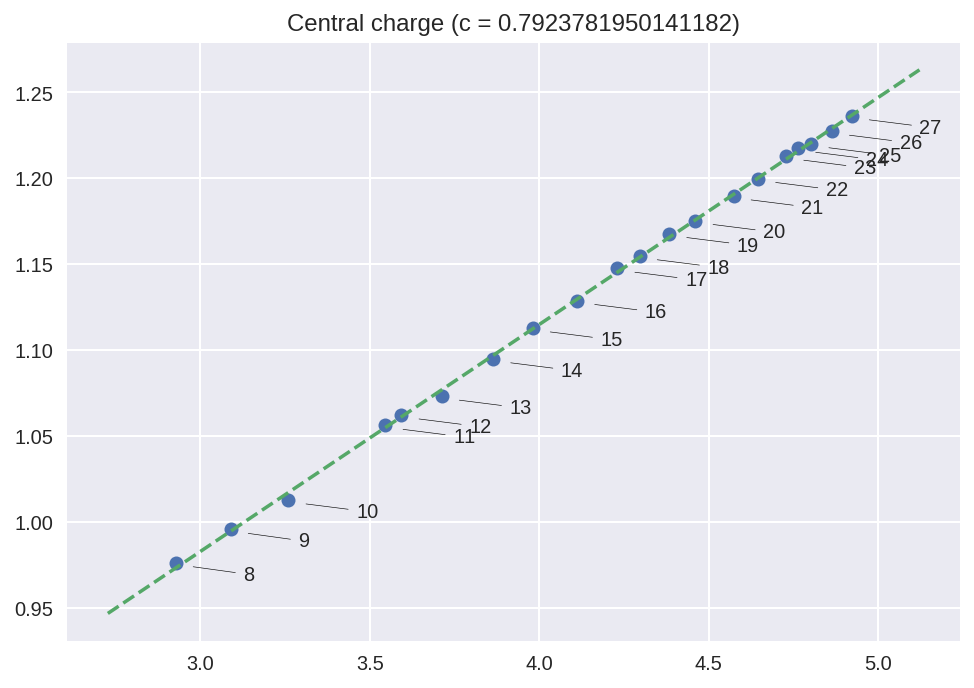
\includegraphics[width=0.45\textwidth]{images/fib-central-charge.png}}
  \caption[中心荷拟合结果]{中心荷拟合结果。横坐标:关联长度的对数 $\log\xi$,纵坐标:纠缠熵 $S_A$。使用的连接维数为 $\chi\in\{8,9,\dots,27\}$。}
  \label{fig:central-charge}
\end{figure}

% \subsection{高度模型}
% TODO: \emph{高度模型} (height model)

\section{MPO 对称性}

在弦网模型的 PEPS 张量网络表示中,弦激发可以理解为由满足\emph{推拉条件} (pulling-through condition) 的矩阵乘积算符 (MPO) 产生。这些 MPO 具有一定的代数结构,任意子则可通过在 MPO 两端放置缺陷张量来产生。MPO 的对称性给出了另外的 $C^*$ 代数结构,其\emph{中心幂等元} (central idempotent) 也对应了输出范畴的不同\emph{拓扑分区} (topological sector),即不同的任意子类型\cite{bultinck2017anyons,williamson2017symmetry,lootens2019cardy,aasen2020topological,sahinoglu2021characterizing}。

\subsection{推拉条件}

弦网模型中的 MPO 张量单元为\footnote{式~\eqref{eq:string-net-mpo}--\eqref{eq:tube-algebra-hermitian-conjugate} 中图片来源:\parencite{williamson2017symmetry}。}:
\begin{equation}
    \vcenter{\hbox{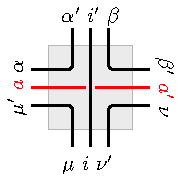
\includegraphics{images/mpo/TCMPO.pdf}}}
  = \delta_{\alpha\alpha'} \delta_{\beta\beta'} \delta_{\mu\mu'} \delta_{\nu\nu'} \delta_{ii'} \delta_{aa'}
    \frac{F^{a\mu i}_{\beta\alpha\nu}}{\sqrt{d_\alpha d_\nu}}.
  \label{eq:string-net-mpo}
\end{equation}
张量的指标都是融合范畴 $\mathcal{C}$ 中的简单对象。由此组成的 MPO 则为
\begin{equation}
    \mathrm{MPO}_a = \, \vcenter{\hbox{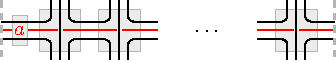
\includegraphics[scale=1.5]{images/mpo/smallTCmpo.pdf}}} \, ,
\end{equation}
其中虚线表示周期性边界条件,而
\begin{equation}
    \vcenter{\hbox{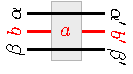
\includegraphics[scale=1.2]{images/mpo/TCMPOclosure.pdf}}}
  = \delta_{\alpha\alpha'} \delta_{\beta\beta'} \delta_{bb'} \delta_{ab}.
\end{equation}
它们之间满足融合规则:
\begin{equation}
  \mathrm{MPO}_a \, \mathrm{MPO}_b = \sum_c N_{ab}^c \, \mathrm{MPO}_c,
\end{equation}
其中 $N_{ab}^c$ 和输入范畴所给出的数据是一致的。通过插入融合张量
\begin{equation}
    \vcenter{\hbox{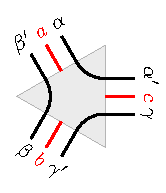
\includegraphics{images/mpo/TCMPOfusion.pdf}}}
  = \delta_{\alpha\alpha'} \delta_{\beta\beta'} \delta_{\gamma\gamma'}
    \left( \frac{d_a d_b}{d_c} \right)^{1/4}
    \frac{F^{ab\gamma}_{\alpha c\beta}}{\sqrt{d_\beta}},
\end{equation}
融合规则也可以表述为
\begin{equation}
    \vcenter{\hbox{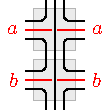
\includegraphics[scale=1.2]{images/mpo/TCMPOmultLHS.pdf}}}
  = \sum_c \delta^c_{ab} \sqrt{\frac{d_c}{d_a d_b}}
    \vcenter{\hbox{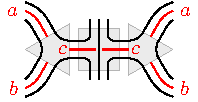
\includegraphics[scale=1.2]{images/mpo/TCMPOmultRHS.pdf}}}.
\end{equation}
不同的缩并顺序对结果的影响由 $F$ 符号给出:
\begin{equation}
    \vcenter{\hbox{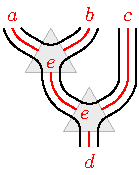
\includegraphics{images/mpo/TCFsymbolLHS.pdf}}} \enspace
  = \sum_f F^{abc}_{def} \enspace
    \vcenter{\hbox{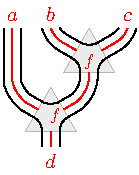
\includegraphics{images/mpo/TCFsymbolRHS.pdf}}}.
\end{equation}

弦网模型的 PEPS 张量网络表示是 \emph{MPO 单射} (MPO-injective) 的,它满足\emph{推拉条件} (pulling-through condition):
\begin{equation}
  \vcenter{\hbox{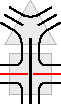
\includegraphics[scale=1.2]{images/mpo/smallTCPullthruLHS.pdf}}}
  \enspace = \enspace
  \vcenter{\hbox{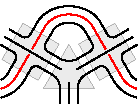
\includegraphics[scale=1.2]{images/mpo/smallTCPullthruRHS.pdf}}},
\end{equation}
即 MPO 可以自由地穿过 PEPS 张量单元。注意到 MPO 和 PEPS 的张量单元可通过同一组 $F$ 符号来确定,因此推拉条件实际上是融合范畴中五边形方程(图~\ref{fig:f-symbols-pentagon-equation})的推论。此时,PEPS 张量网络可以视为背景,而其中的 $\mathrm{MPO}_\psi$ 则表示对应的弦算符(见图~\ref{fig:peps-mpo})。

\begin{figure}[htb]
  \[
    \vcenter{\hbox{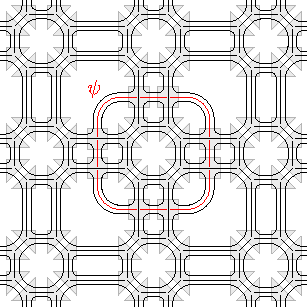
\includegraphics[scale=1.2]{images/mpo/TCpsiPEPS.pdf}}}
    \quad \to \quad
    \vcenter{\hbox{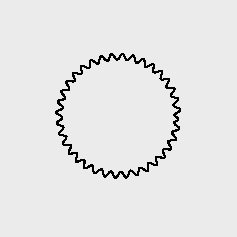
\includegraphics[scale=1.2]{images/mpo/TCpsibackground.pdf}}}
  \]
  \caption[PEPS 张量网络与其中的 MPO]{PEPS 张量网络与其中的 MPO。图片来源:\parencite{williamson2017symmetry}。}
  \label{fig:peps-mpo}
\end{figure}

% TODO: MPO and topological properties

\subsection{管状代数与中心幂等元}
\label{subsec:tube-algebra-idempotents}

考虑一个圆柱上的 PEPS 张量网络,对于其上的弦算符 (MPO),我们可以取下面的基来描述:
\begin{equation}
    \mathcal{T}^{s}_{pqr}
  = \, \vcenter{\hbox{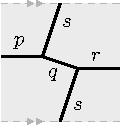
\includegraphics{images/mpo/Tube0.pdf}}} \,
  = \vcenter{\hbox{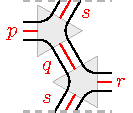
\includegraphics{images/mpo/TCtensortube.pdf}}}.
\end{equation}
它们的乘法和 Hermitian 共轭分别为
\begin{align}
     \mathcal{T}^{s}_{pqr} \mathcal{T}^{s'}_{p'q'r'}
  &= \delta_{rp'} \, \vcenter{\hbox{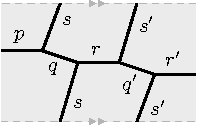
\includegraphics{images/mpo/TCTubemult.pdf}}} \notag \\
  &= \delta_{rp'} \sum_{q''s''} F^{sqs'}_{q'rq''} F^{q''s's}_{pqs''} F^{s'sq''}_{r'q's''}
     \sqrt{\frac{d_s d_{s'}}{d_{s''}}} \mathcal{T}^{s''}_{pq''r'}, \\
     \bigl( \mathcal{T}^{s}_{pqr} \bigr)^\dagger
  &= \, \vcenter{\hbox{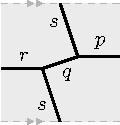
\includegraphics{images/mpo/TCTubedagger.pdf}}} \,
   = \sqrt{\frac{d_p}{d_r}} \sum_{q'} F^{srs}_{pqq'} \mathcal{T}^{s}_{rq'p}.
  \label{eq:tube-algebra-hermitian-conjugate}
\end{align}
由此可见,这些基关于乘法和 Hermitian 共轭都是封闭的,因而它们构成了一个 $C^*$ 代数,称为 \emph{Ocneanu 管状代数} (Ocneanu's tube algebra)\cite{evans1995ocneanu,evans1998quantum}。

管状代数可以被分块对角化,其中的每一块上的投影算符对应一个\emph{不可约中心幂等元} (irreducible central idempotent)。从范畴论的角度来看,这些中心幂等元构成了一个新的范畴,它对应了输入范畴 $\mathcal{C}$ 的 \emph{Drinfel'd 中心} (Drinfel'd center) $\mathcal{Z}(\mathcal{C})$。而从拓扑序的角度来看,它们则对应了不同的\emph{拓扑分区} (topological sectors)\cite{lan2014topological,bultinck2017anyons,williamson2017symmetry,vanhove2018mapping}。

中心幂等元可以表示为管状代数中基的线性组合:
\begin{equation}
  \mathcal{P}_{i} = \frac{1}{D^2} \sum_{pqrs} t^i_{pqrs} \mathcal{T}^{s}_{pqr},
\end{equation}
其中 $D$ 为总量子维数,而系数 $t^i_{pqrs}$ 可根据 $\mathcal{P}_{i}$ 满足的约束条件来求解:
\begin{equation}
  \mathcal{P}_{i} \mathcal{P}_{j} = \delta_{ij} \mathcal{P}_{i}, \quad
  \mathcal{P}_{i}^\dagger = \mathcal{P}_{i}, \quad
  \mathcal{T}^{s}_{pqr} \mathcal{P}_{i} = \mathcal{P}_{i} \mathcal{T}^{s}_{pqr}.
\end{equation}
以包含 $\1$、$\tau$ 两种任意子的 Fibonacci 模型为例\cite{bultinck2017anyons},它的中心幂等元共有 4 个:
\begin{equation}
  \begin{aligned}
    \mathcal{P}_{1} &= \frac{1}{\sqrt5} \left(
      \frac{1}{\varphi} \mathcal{T}^{\1}_{\1\1\1} + \sqrt{\varphi} \mathcal{T}^{\tau}_{\1\tau\1}
    \right), \\
    \mathcal{P}_{2} &= \frac{1}{\sqrt5} \left(
      \frac{1}{\varphi} \mathcal{T}^{\1}_{\tau\tau\tau} + \frac{1}{\sqrt{\varphi}} \ee^{-4\pi\ii/5} \mathcal{T}^{\tau}_{\tau\1\tau} + \ee^{ 3\pi\ii/5} \mathcal{T}^{\tau}_{\tau\tau\tau}
    \right), \\
    \mathcal{P}_{3} &= \frac{1}{\sqrt5} \left(
      \frac{1}{\varphi} \mathcal{T}^{\1}_{\tau\tau\tau} + \frac{1}{\sqrt{\varphi}} \ee^{ 4\pi\ii/5} \mathcal{T}^{\tau}_{\tau\1\tau} + \ee^{-3\pi\ii/5} \mathcal{T}^{\tau}_{\tau\tau\tau}
    \right), \\
    \mathcal{P}_{4} &= \frac{1}{\sqrt5} \left(
      \varphi \mathcal{T}^{\1}_{\1\1\1} + \mathcal{T}^{\1}_{\tau\tau\tau} - \sqrt{\varphi} \mathcal{T}^{\tau}_{\1\tau\1} + \sqrt{\varphi} \mathcal{T}^{\tau}_{\tau\1\tau} + \frac{1}{\varphi} \mathcal{T}^{\tau}_{\tau\tau\tau}
    \right),
  \end{aligned}
  \label{eq:fib-idempotents}
\end{equation}
分别对应了 doubled Fibonacci(即 Fibonacci 的 Drinfel'd 中心)中的 4 种任意子:
\begin{equation}
  \mathcal{P}_{1} \mapsto (\1, \1), \quad
  \mathcal{P}_{2} \mapsto (\1, \bar{\tau}), \quad
  \mathcal{P}_{3} \mapsto (\tau, \1), \quad
  \mathcal{P}_{4} \mapsto (\tau, \bar{\tau}),
\end{equation}
相应的拓扑自旋分别为
\begin{equation}
  h_1 = 0, \quad h_2 = -\frac45, \quad h_3 = \frac45, \quad h_4 = 0.
\end{equation}

\section{全息张量网络}
\label{sec:holographic-tensor-network}

% 首先,我们将奇异关联子的概念推广到了任意维度($1\leqslant D\leqslant 3$),并且给出了一种系统的方法用以构造配分函数和搜寻临界点。我们的方法基于对 $\bra{\Omega}$ 的理解。根据融合范畴 $\mathcal{C}$ 及其对应的范畴对称性 $\mathcal{Z}(\mathcal{C})$,我们可以构造一套重整化算符,并将其作为全息张量网络。它可以对拓扑序的基态波函数 $\ket{\Psi}$ 进行粗粒近似。为了使 $\langle\Omega|\Psi\rangle$ 能够表示对应共形场论的配分函数,$\bra{\Omega}$ 需要是重整化算符的本征态。实际上,带有范畴对称性 $\mathcal{Z}(\mathcal{C})$ 的 $D$ 维共形场论,也就相当于由 $D+1$ 维拓扑序所确定的重整化算符的本征态。我们发现,对于中心为 $\mathcal{Z}(\mathcal{C})$ 的输入范畴 $\mathcal{C}$,其中的每一个 \emph{Frobenius 代数} (Frobenius algebra) 都确定了一个 $D+1$ 维的格点拓扑模型,它们对应了重整化算符的本征态,能给出一个 $D$ 维的对称 TQFT,而 CFT 就位于这些 TQFT 的相变点处。我们可以在相变点两侧各取一个 Frobenius 代数,而描述 CFT 的边界条件即可通过这两个 Frobenius 代数对应的边界条件插值得到。而在远离 CFT 不动点处,重复作用这些重整化算符将会给出 $\mathcal{C}$ 的 Frobenius 代数。从数值角度上看,当我们对三维的配分函数不断作用重整化算符时,实际上也就相当于实现了类似于三维 TRG 算法的操作。这种全息张量网络与 $p$-adic 张量网络也存在相似之处。后者中的张量单元由 $p$-adic CFT 融合范畴中结合代数的乘积/余积结构给出,而前者则需要利用 $D-1$ 维融合范畴中的 Frobenius 代数结构,这正是结合代数的自然推广。

我们在 \ref{sec:strange-correlator} 节中所介绍的奇异关联子也可以被推广到任意维度。对于一个 $D+1$ 维的拓扑序,它可以用一个 $D+1$ 维球 $B^{D+1}$ 上的融合范畴 $\mathcal{C}$ 来描述,其基态波函数为 $\ket{\Psi}$。指定 $D$ 维球面 $S^D$ 上的边界条件,就相当于将 $\ket{\Psi}$ 与某一直积态 $\ket{\Omega}$ 作内积,即
\begin{equation}
  Z(\Omega, \mathcal{C}) = \langle \Omega|\Psi \rangle.
\end{equation}
由于 $\ket{\Psi}$ 是一个拓扑序的基态波函数,它应该在标度变换下保持不变。设标度变换可由重整化算符 $\mathcal{H}_{\mathcal{C}}$ 生成,则可有
\begin{equation}
  Z(\Omega, \mathcal{C}) = \langle \Omega | \exp(z\mathcal{H}_{\mathcal{C}}) | \Psi \rangle,
\end{equation}
其中 $z$ 是重整化坐标。考虑到 $Z(\Omega, \mathcal{C})$ 描述了一个 $D$ 维的拓扑 / 共形系统,因此
\begin{equation}
  \bra{\Omega} \exp(z\mathcal{H}_{\mathcal{C}}) = \bra{\Omega},
  \label{eq:rg-operator}
\end{equation}
即配分函数的构建可以转化为关于 $\mathcal{H}_{\mathcal{C}}$ 的本征值问题。重整化算符 $\mathcal{H}_{\mathcal{C}}$ 可以将体($D+1$ 维球 $B^{D+1}$)与不同格点标度下的边界($D$ 维球面 $S^D$)联系起来,因而也就能够用来构建一套\emph{全息张量网络} (holographic tensor network)。下面我们讨论几个不同维度中的具体例子。

\subsection{1+1 维:基于 Dijkgraaf--Witten 理论}
\label{subsec:holographic-tensor-network-1+1d}

我们首先考察由群 $G$ 所刻画的 1+1 维 Dijkgraaf--Witten 模型\cite{dijkgraaf1990topological}。为了计算二维流形 $M^2$ 上的路径积分,我们先对其进行三角剖分,每个三角形对应于
\begin{equation}
  \alpha_2(g_1, g_2) \in H^2 \bigl( G, U(1) \bigr),
\end{equation}
其中 $H^2$ 是群上同调,而 $g_i\in G$ 满足群乘法
\begin{equation}
  g_1 \times g_2 = g_3.
\end{equation}
如图~\ref{fig:dw-triangle} 所示,群乘法也决定了三角形的定向。我们选取圆盘作为底流形,则路径积分将会在圆 $S^1$ 上给出相应二维模型的基态波函数。最简单的三角剖分如图~\ref{fig:dw-triangulation} 所示,它可以表示为一个矩阵乘积态:
\begin{equation}
    \ket{\Psi}_G
  = \sum_{\{g_i\}} \sum_{\{h_i\}}
    \bigl[ \cdots \tau_{h_i h_{i+1}}(g_i) \, \tau_{h_{i+1} h_{i+2}}(g_{i+1}) \cdots \bigr]
    \ket{\dots, g_i, g_{i+1}, \dots},
\end{equation}
其中
\begin{equation}
  \tau_{h_i h_{i+1}}(g) = \alpha^\varepsilon(h_i, h_{i+1}) \, \delta_{g, h_i h_{i+1}},
\end{equation}
而 $\varepsilon=\pm1$ 则根据三角形的定向来确定。

\begin{figure}[htb]
  \centering
  \subcaptionbox{\label{fig:dw-triangle}}{%
    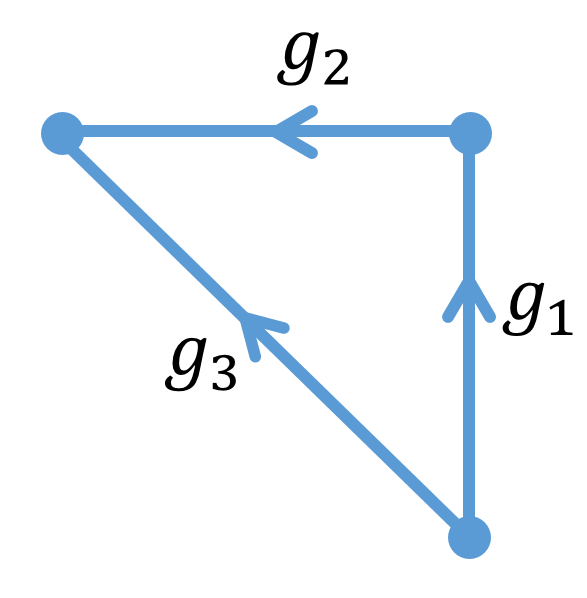
\includegraphics[width=0.2\textwidth]{images/holographic/dw-triangle.png}} \quad
  \subcaptionbox{\label{fig:dw-triangulation}}{%
    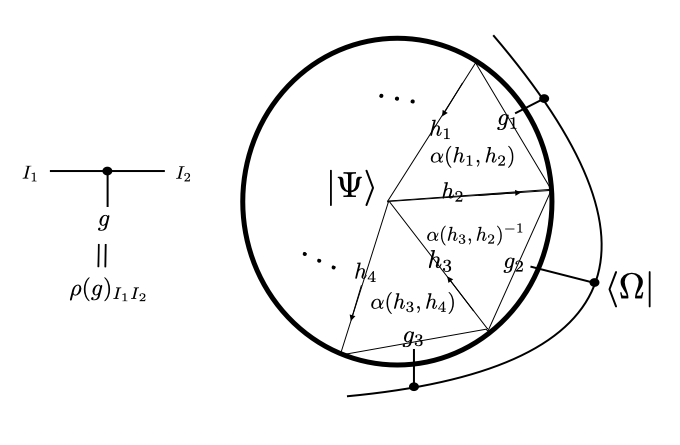
\includegraphics[width=0.5\textwidth]{images/holographic/dw-triangulation.png}}
  \caption[1+1 维 Dijkgraaf--Witten 模型的三角剖分]{1+1 维 Dijkgraaf--Witten 模型的三角剖分。(a) Dijkgraaf--Witten 模型中,三角形对应了 $\alpha_2(g_1, g_2)$,而其定向则由群乘法决定。(b) 圆盘上最简单的三角剖分及对应 $\bra{\Omega}$ 的张量网络表示。图片来源:\parencite{chen2022exact}。}
\end{figure}

这些三角形满足结合条件:
\begin{equation}
  \alpha(g_1, g_2) \, \alpha(g_1 g_2, g_3) = \alpha(g_1, g_2 g_3) \, \alpha(g_2, g_3).
  \label{eq:associativity-condition}
\end{equation}
据此可将边界 $S^1$ 上的 $2N$ 条边变为 $N$ 条边。于是我们就得到了树状结构的算符 $U_N(G,\alpha)$,它联系起了长度为 $2N$ 和 $N$ 的两条边界。我们取
\begin{equation}
  \exp(z\mathcal{H}) \to U(G,\alpha) \coloneq \lim_{N\to\infty} U_N(G,\alpha).
\end{equation}
根据式~\eqref{eq:rg-operator},$U(G,\alpha)$ 的本征态 $\bra{\Omega}$ 即给出了标度不变的配分函数 $Z(\Omega,G)$,并且具有全局对称性 $G$[图~\ref{fig:rg-1+1d}]。

\begin{figure}[htb]
  \centering
  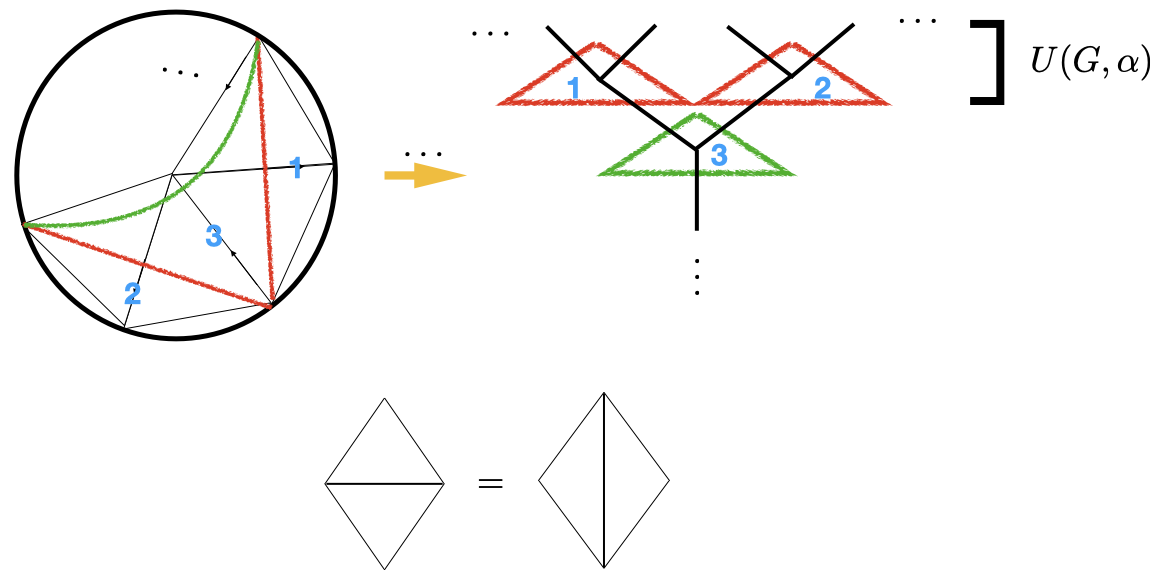
\includegraphics[width=0.6\textwidth]{images/holographic/rg-1+1d.png}
  \caption[结合条件与树状结构的张量网络]{重复利用式~\eqref{eq:associativity-condition} 中的结合条件(图片下半部分),圆盘的三角剖分可以被改写为一个树状结构的张量网络。图片来源:\parencite{chen2022exact}。}
  \label{fig:rg-1+1d}
\end{figure}

简单起见,我们只考虑 $H^2$ 中的平凡元素,即 $\alpha(g_1, g_2)=1$。此时,$U(G,1)$ 的本征态 $\bra{\Omega}$ 可以写成 MPS 的形式,
\begin{equation}
    \bra{\Omega}
  = \sum_{\{g\}} \tr\bigl[ \cdots \rho(g_i) \, \rho(g_{i+1}) \cdots \bigr]
    \bra{\dots, g_i, g_{i+1}, \dots},
\end{equation}
其中 $\rho$ 是群 $G$ 的表示矩阵,它满足
\begin{equation}
  \bigl[ \rho(g_1) \, \rho(g_2) \bigr]_{ij} = \sum_s \rho_{is}(g_1) \, \rho_{sj}(g_2) = \rho_{ij}(g_1 g_2).
\end{equation}
此外还可以证明,重整化算符的一般形式可以分解为 $G$ 表示的直积:
\begin{equation}
  \rho(g) = \bigoplus_\mu \rho^\mu(g),
\end{equation}
式中 $\mu$ 标记了群 $G$ 的不同不可约表示。这样我们得到的配分函数 $Z=\langle\Omega|\Psi\rangle_G$ 就可以表示为一组张量
\begin{equation}
  T_{IJ}(g) \coloneq \rho_{ij}(g) \, \alpha^\varepsilon(h,k) \, \delta_{g, hk}, \quad
  I = (i,h), \, J = (j,k)
\end{equation}
的缩并形式,而其中所有的关联函数都会以指数级衰减,这与一维系统的性质也是相符的。

\subsection{2+1 维:基于 Turaev--Viro 理论}
\label{subsec:holographic-tensor-network-2+1d}

2+1 维的情况实际上就对应了奇异关联子的原始定义(\ref{sec:strange-correlator} 节)。我们考虑一个对应于融合范畴 $\mathcal{C}$ 的 Turaev--Viro TQFT。对于球面 $S^2$ 上的基态波函数,它可由一个三维球 $B^3$ 上的路径积分给出,利用三角剖分则可将 $B^3$ 变为四面体的形式。方便起见,我们不妨令剖分得到的截面与图~\ref{fig:dw-triangulation} 中的情形相同,即球面 $S^2$ 被三角形所覆盖,而三角形的每个顶点都有一条边延伸至球心。每条边被赋予了 $\mathcal{C}$ 中的一个对象,而每个四面体则被赋予一个四面体符号的值,它由 $\mathcal{C}$ 中对象的融合关系所定义。这样,我们就获得了基态波函数的张量网络表示(见图~\ref{fig:ground-state-wave-function},也可参考 \ref{subsec:string-net-ground-state} 小节)。这些四面体符号之间满足的关系在 \ref{subsec:tetrahedral-symmetry} 小节中也已经讨论过了,此处我们重新整理在图~\ref{fig:tetrahedra-symbols} 中。

\begin{figure}[htb]
  \centering
  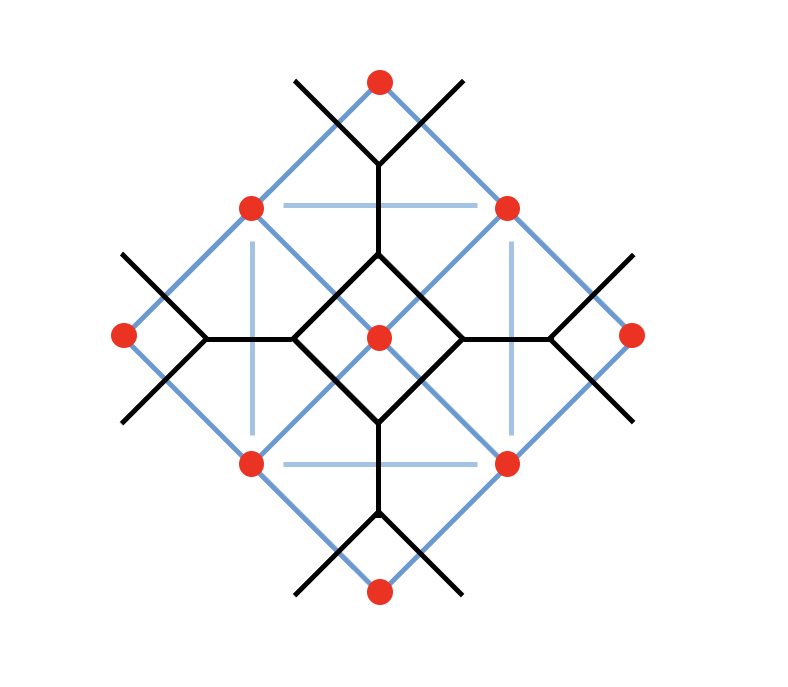
\includegraphics[width=0.4\textwidth]{images/holographic/ground-state-wave-function.png}
  \caption[2+1 维 Turaev--Viro TQFT 中基态波函数的张量网络表示]{2+1 维 Turaev--Viro TQFT 中基态波函数的张量网络表示。蓝线代表物理指标,而红点代表垂直于 $S^2$ 面的辅助指标,它们对应了 $\mathcal{C}$ 中对象按量子维数的加权和。图片来源:\parencite{chen2022exact}。}
  \label{fig:ground-state-wave-function}
\end{figure}

\begin{figure}[htb]
  \centering
  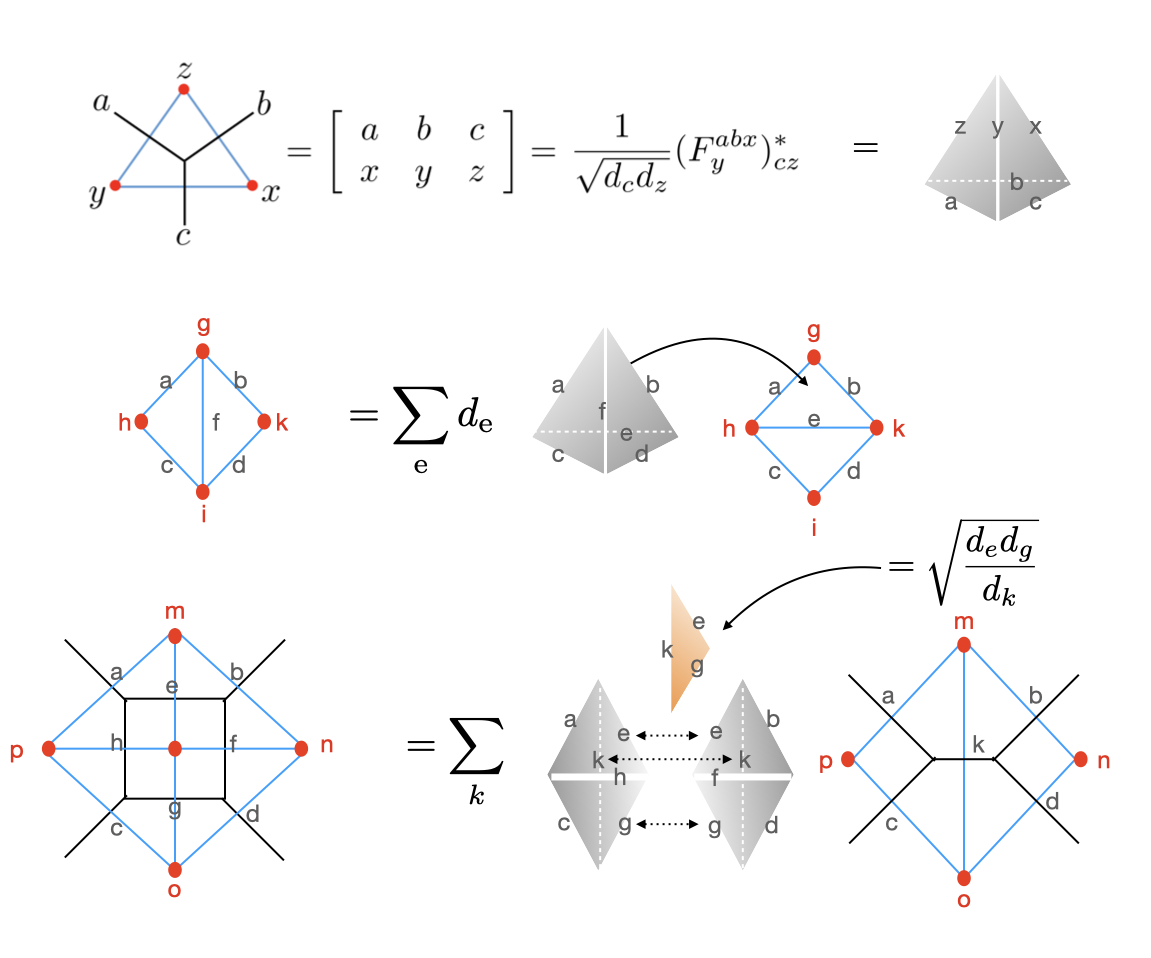
\includegraphics[width=0.9\textwidth]{images/holographic/tetrahedra-symbols.png}
  \caption[四面体符号]{张量单元的取值由四面体符号给出,而五边形方程则相当于在原来四面体的表面(即两个三角形)上叠加一个新的四面体,从而改变了表面的三角剖分。图片来源:\parencite{chen2022exact}。}
  \label{fig:tetrahedra-symbols}
\end{figure}

与 1+1 维的情况类似,在 2+1 维中重整化算符同样通过连接两个不同格点间距的边界来构造。如图~\ref{fig:rg-2+1d} 所示,我们可以利用一系列的 $F$ 移动及相应的变换关系(图~\ref{fig:tetrahedra-symbols})来得到重整化算符 $U(\mathcal{C})$\cite{vanhove2018mapping}。它可以表示为一系列四面体的组合,并会将第 $N$ 次粗粒近似的波函数映射到第 $N+1$ 次上。可以发现,$U(\mathcal{C})$ 完全由融合范畴 $\mathcal{C}$ 中的数据所决定,而重复作用 $U(\mathcal{C})$ 将得到 Euclidean AdS 空间的一个离散化表示。

\begin{figure}[htb]
  \centering
  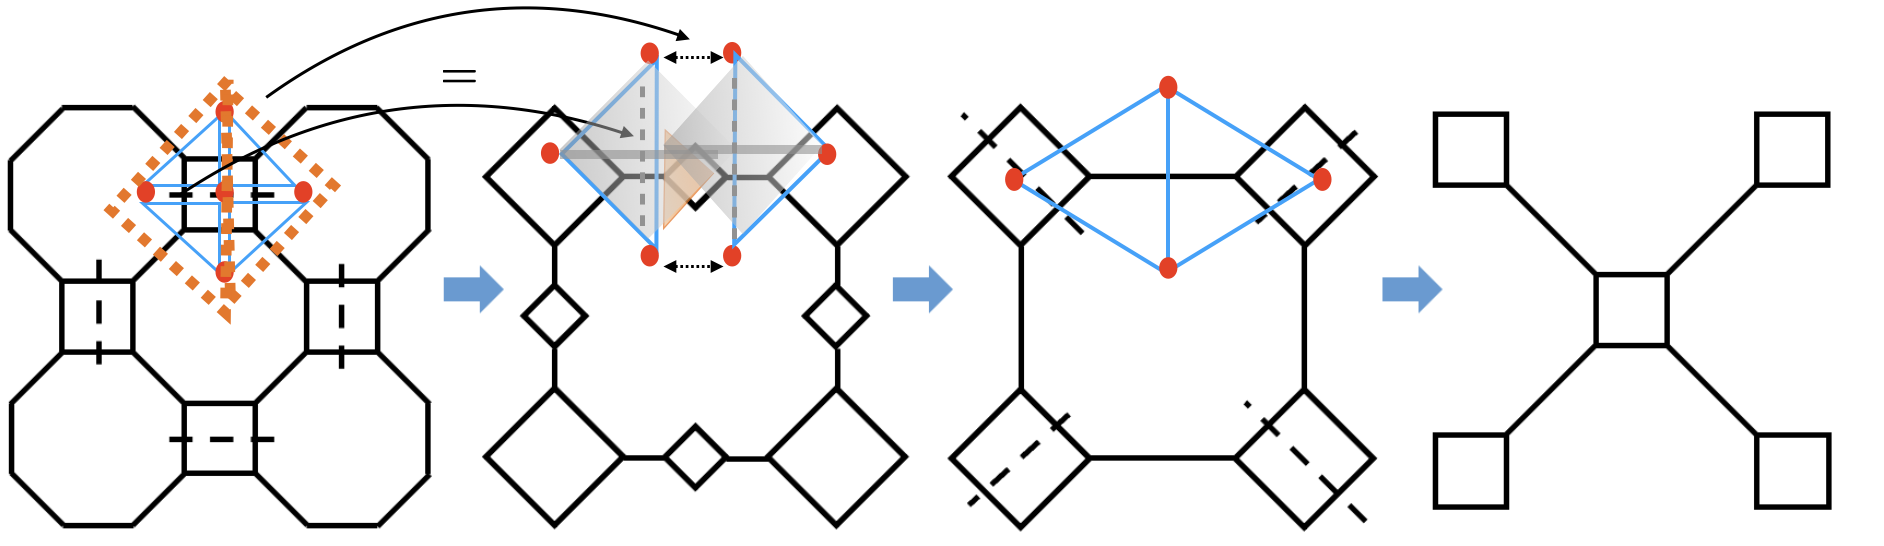
\includegraphics[width=0.9\textwidth]{images/holographic/rg-2+1d.png}
  \caption[利用五边形方程来实现粗粒近似]{利用五边形方程来实现粗粒近似。重整化算符可以视为一系列四面体的组合,例如第一幅图中的四个三角形在作用一组四面体后(标记为灰色),就变为了两个三角形。图片来源:\parencite{chen2022exact}。}
  \label{fig:rg-2+1d}
\end{figure}

% TODO: Frobenius Algebra

特别值得关注的是位于临界点处的配分函数。当非对易的拓扑对称性同时守恒时,即为临界点。
由于配分函数 $Z(\mathcal{C})$ 是局域的,因而 $\bra{\Omega}$ 可以表示为一个 PEPS 张量网络。我们将张量单元 $T^{a_1 a_2 a_3}_{I_1 I_2 I_3}$ 取在三角形上,其中 $a_i\in\mathcal{C}$ 为物理指标,而 $I_i$ 为辅助指标,连接维数为 $\chi$。在重整化开始前,$\bra{\Omega}$ 是一个直积态,即所有 $I_i$ 都是平凡的;随着重整化的进行,相应的数据会“流入” $I_i$,得到非平凡的 PEPS 结构。

原则上,$T^{a_1 a_2 a_3}_{I_1 I_2 I_3}$ 的具体形式可以根据拓扑序中开弦算符按幂律衰减的性质来确定。然而,幂律衰减意味着 $\chi$ 会随着系统尺寸的增大而增大;对于无限系统而言,应有 $\chi\to\infty$。这在实际计算中显然是无法实现的。为此,我们采取另一套方案来获取临界点数据。考虑单个重整化步骤 $\bra{\Omega(T)}U(\mathcal{C})$。如图~\ref{fig:rg-2+1d} 所示,四个三角形被映射到了两个三角形,而它们之间带有纠缠的边界条件。对于这种边界,我们可以通过奇异值分解 (SVD) 把它编码到辅助指标 $I_i$ 上,并且把相应的连接维数控制在合理范围内。如图~\ref{fig:rg-2+1d-blocking},这时四个 $T$ 的乘积就可以被改写为两个新张量 $\tilde{T}$ 的缩并。

\begin{figure}[htb]
  \centering
  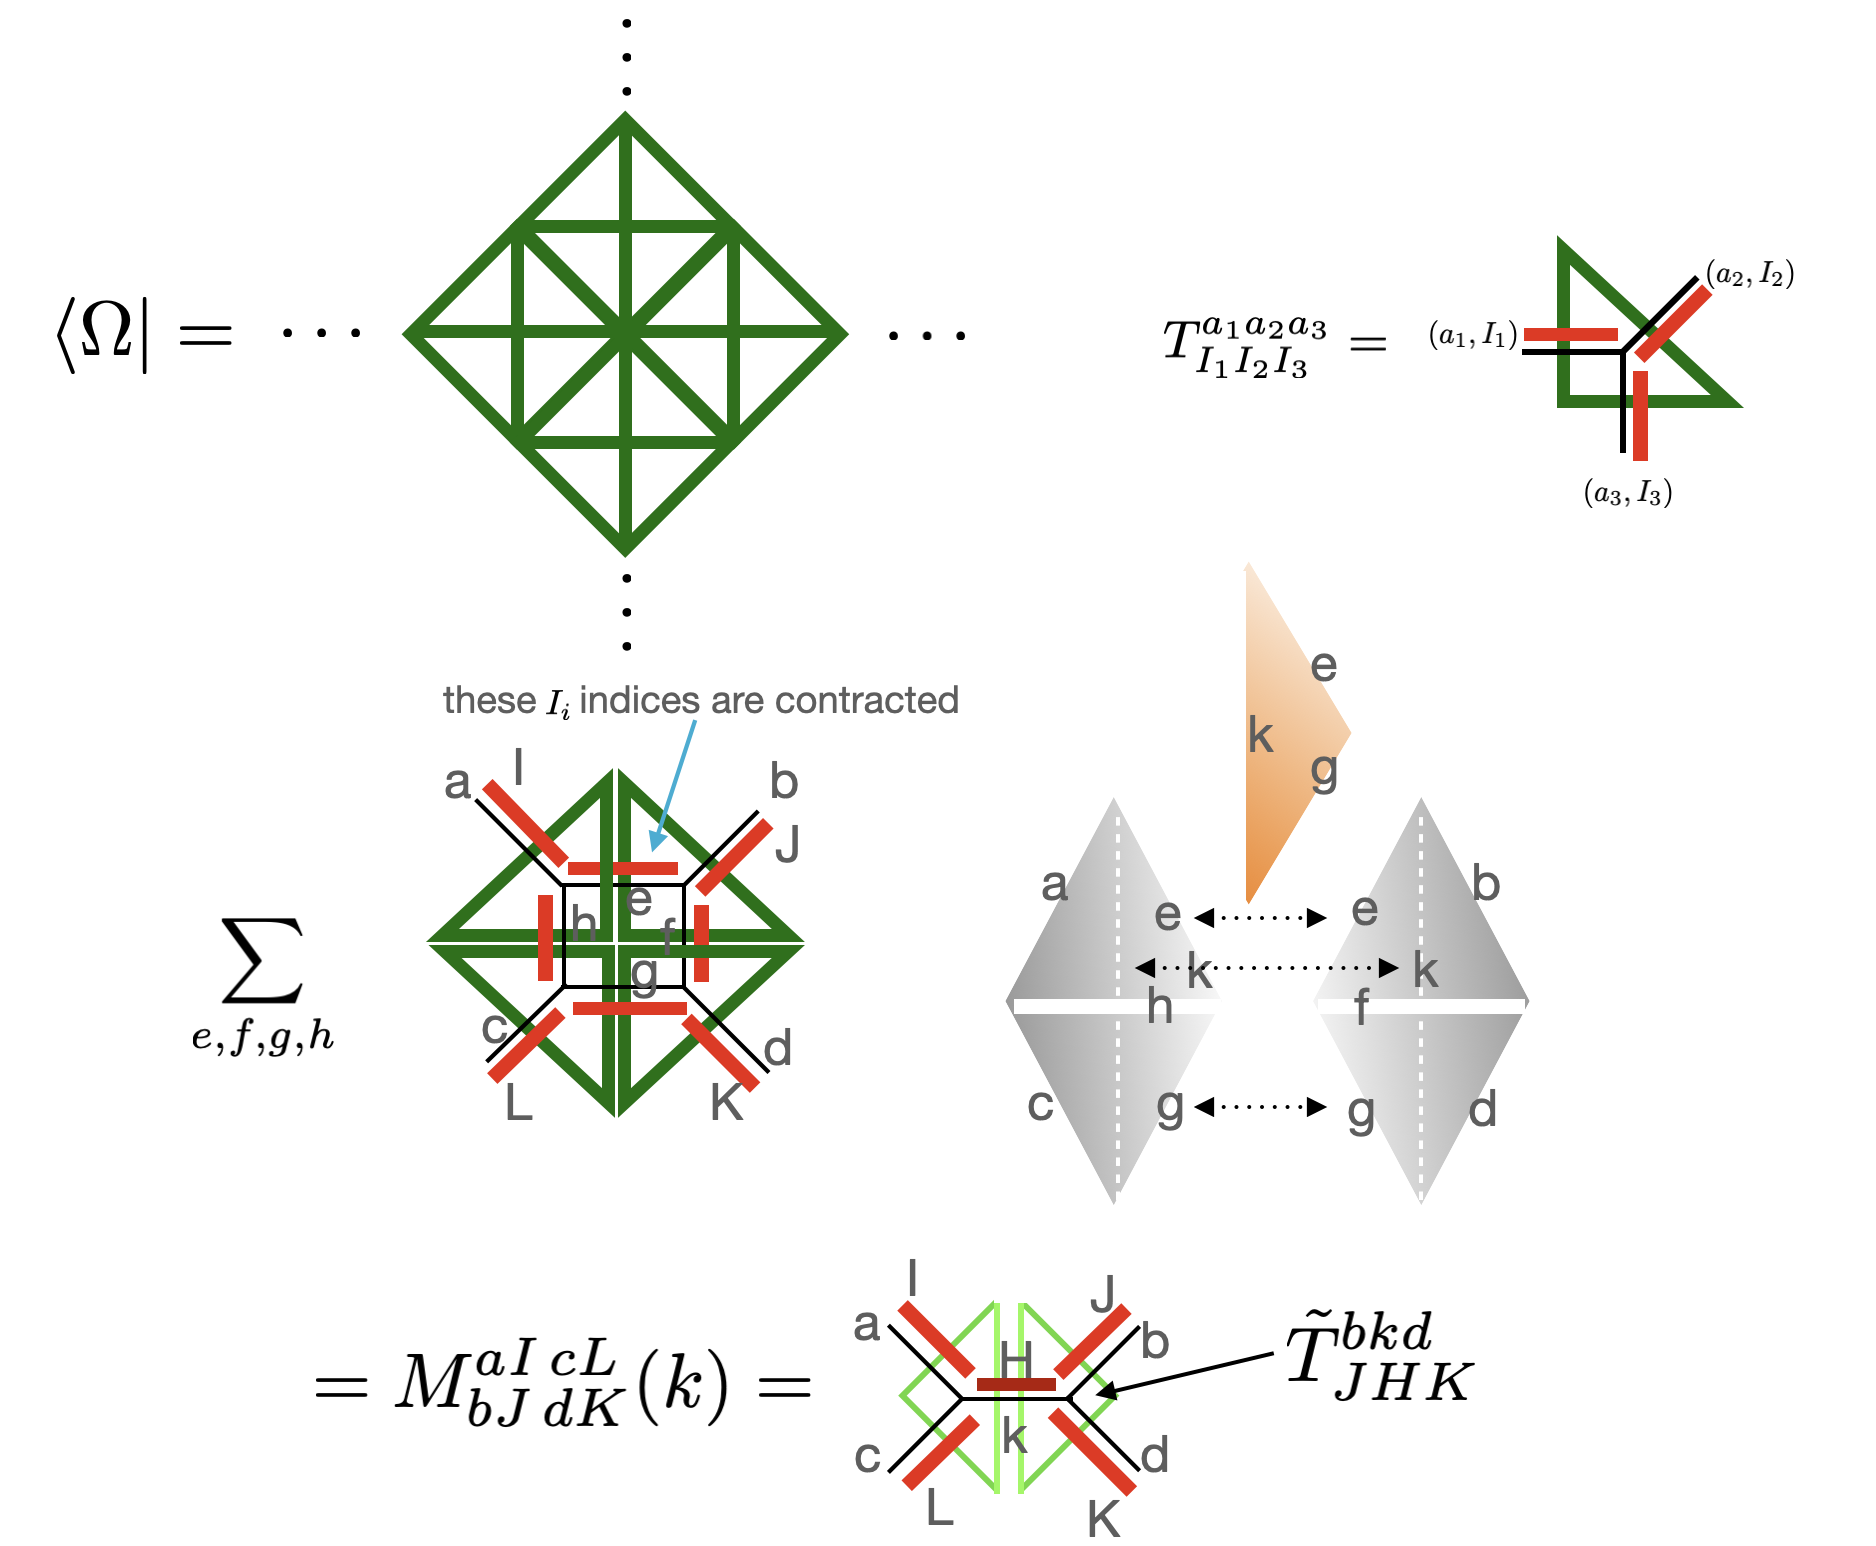
\includegraphics[width=0.8\textwidth]{images/holographic/rg-2+1d-blocking.png}
  \caption[边界态 $\bra{\Omega}$ 的 PEPS 张量网络表示]{上图为边界态 $\bra{\Omega}$ 的 PEPS 张量网络表示,其指标位于三角形的边上。每条边都有两个指标,一个是物理指标 $a_i\in\mathcal{C}$,另一个是连接维数为 $\chi$ 的辅助指标 $I_i$。在下图中,我们利用 SVD 把张量 $M(k)$ 分解为两个张量 $\tilde{T}$ 的缩并。指标 $H$(标记为红色)在生成时,连接维数为 $\chi^2$,但我们会将其截断为 $\chi$ 以使得重整化过程得以持续。图片来源:\parencite{chen2022exact}。}
  \label{fig:rg-2+1d-blocking}
\end{figure}

需要注意的是,对于有限大小的 $\chi$,临界点是不稳定的,而从重整化过程中获得的 $T$ 序列最终会流向某个拓扑不动点。因此我们认为,在重整化过程中,如果观察到 $T$ 开始向拓扑不动点的方向收敛,即达到了临界点。而对于固定的 $\chi$,总能利用这种方式找到一组 $T$ 使其最接近临界态。

% TODO: \mathfrak{su}(2)_k / SU(2)_k / A_{k+1}

接下来我们以 $\mathcal{A}_{k+1}$ 模型(见 \ref{subsec:a-k+1-category} 小节)为例给出一些具体的数值计算结果。如图~\ref{fig:a-k+1-boundary-condition} 所示,$\mathcal{A}_{k+1}$ 中的边界态可以取为
\begin{equation}
  \bra{\Omega} = \sum_{\{a\}} \prod_{a_1, a_2, a_3} T^{a_1, a_2, a_3} \bra{\{a\}},
\end{equation}
其中三角形上的 $T$ 张量为
\begin{equation}
  T^{a_1, a_2, a_3} = \begin{cases}
    1, & a_1 = a_3 = \frac12, \, a_2 = 0; \\
    r, & a_1 = a_3 = \frac12, \, a_2 = 1; \\
    0, & \text{otherwise}.
  \end{cases}
\end{equation}

\begin{figure}[htb]
  \centering
  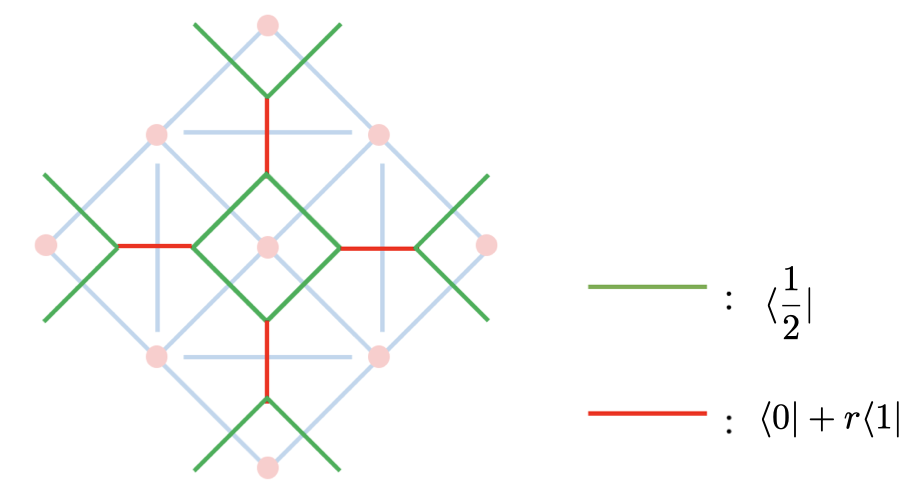
\includegraphics[width=0.5\textwidth]{images/holographic/a-k+1-boundary-condition.png}
  \caption[$\mathcal{A}_{k+1}$ 模型中的边界条件]{$\mathcal{A}_{k+1}$ 模型中的边界条件。$k=2$ 时 $\mathcal{A}_{k+1}$ 等价于 Ising 模型,因而有 $r=\ee^{-2\beta}$。与图~\ref{fig:rg-2+1d-blocking} 相对比,此处的辅助指标 $I_i$ 是平凡的。图片来源:\parencite{chen2022exact}。}
  \label{fig:a-k+1-boundary-condition}
\end{figure}

通过重复作用重整化算符,我们可以让 $T$ 收敛到不动点。作为最粗糙的近似,这里只取连接维数 $\chi=1$。计算结果表明,对于较小的 $r$,不动点张量包含唯一非零分量 $T^{000}$,这对应了可分 Frobenius 代数 $\mathcal{A}_0=\{0\}$;而对于较大的 $r$,不动点张量的非零分量为 $T^{000}=T^{110}=T^{101}=T^{011}$,$k>2$ 时还存在 $T^{111}$,它们的比值为
\begin{equation}
  \frac{T^{000}}{T^{111}} \simeq \begin{cases}
    1.43463, & k = 3; \\
    1.18921, & k = 4.
  \end{cases}
\end{equation}
这与通过可分 Frobenius 代数 $\mathcal{A}_1=\{0,1\}$ 得到的精确值
\begin{equation}
  \frac{T^{000}}{T^{111}} = \frac{\sqrt[4]{2\cos\left(\frac{2\pi}{k+2}\right) + 1}}{\sqrt{2\cos\left(\frac{2\pi}{k+2}\right)}}, \quad
  k > 2
\end{equation}
是相符的。我们还可以得到临界耦合常数 $r_{\text{c}}(k)$(图~\ref{fig:a-k+1-coupling}),这与利用 Kramers--Wannar 对偶得到的精确值
\begin{equation}
  r_{\text{c}} = \frac{\sqrt[4]{2\cos\left(\frac{2\pi}{k+2}\right) + 1}}{\sqrt{2\cos\left(\frac{\pi}{k+2}\right) + 1}}
\end{equation}
也是基本符合的(至一位有效数字)。

\begin{figure}[htb]
  \centering
  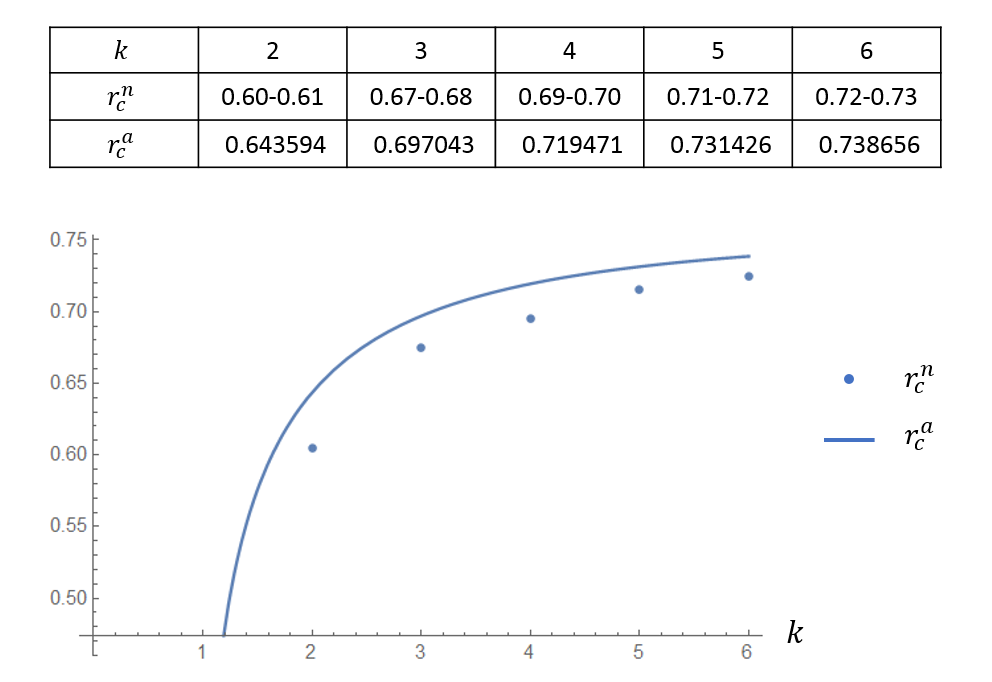
\includegraphics[width=0.6\textwidth]{images/holographic/a-k+1-coupling.png}
  \caption[$\mathcal{A}_{k+1}$ 模型中的临界耦合常数]{$\mathcal{A}_{k+1}$ 模型中的临界耦合常数,这里 $r^{\text{a}}_{\text{c}}$ 和 $r^{\text{n}}_{\text{c}}$ 分别代表理论结果和数值模拟结果。它们符合的程度大致为一位有效数字。图片来源:\parencite{chen2022exact}。}
  \label{fig:a-k+1-coupling}
\end{figure}

\subsection{3+1 维概述}

类似地,三维配分函数也可通过 3+1 维 TQFT 基态波函数与对应的奇异关联子获得。对于 3+1 维 TQFT 而言,输入数据是 \emph{2-融合范畴} (2-fusion category)\cite{lan2018classification,lan2019classification,johnson2021dimensional,johnson2022classification},而相应张量网络的构建块是\emph{四维单形} (4-simplex)。此时,边会被赋予 2-范畴中的对象,面会被赋予 1-态射,而三维单形则会被赋予 2-态射。

3+1 维 TQFT 基态波函数的张量网络表示是 2+1 维的自然推广,它可由以三维球面 $S^3$ 为边界的四维球 $B^4$ 中的路径积分获得。边界 $S^3$ 可被三角剖分为一系列的三维单形,它们共享的指标则位于四维球 $B^4$ 的球心[即图~\ref{fig:dw-triangulation} 的高维推广]。在张量网络中,这些构建块可以表示为四面体的形式,其边和面上都带有指标。波函数则相当于把这些四面体铺满三维边界,并对共享的指标求和。

具体来说,三维边界由一系列小正方体填充,每个正方体可继续分为 6 个四面体,而顶点则被 8 个正方体共享[图~\ref{fig:3+1d-cube-1}]\cite{delcamp2021tensor}。注意这样的正方体单元并不是平移不变的,最小可重复的填充单元需要 $2\times2\times2$ 个小正方体[图~\ref{fig:3+1d-cube-2}]。

\begin{figure}[htb]
  \centering
  \subcaptionbox{\label{fig:3+1d-cube-1}}{%
    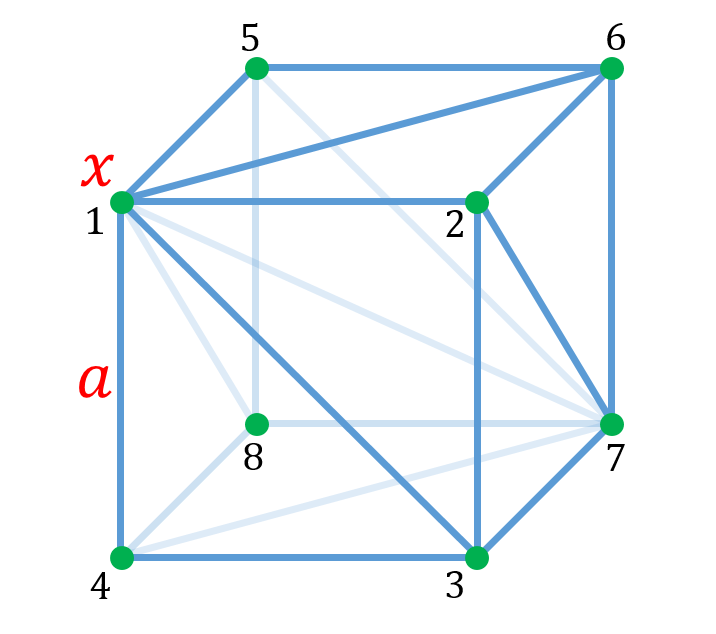
\includegraphics[width=0.25\textwidth]{images/holographic/3+1d-cube-1.png}} \quad
  \subcaptionbox{\label{fig:3+1d-cube-2}}{%
    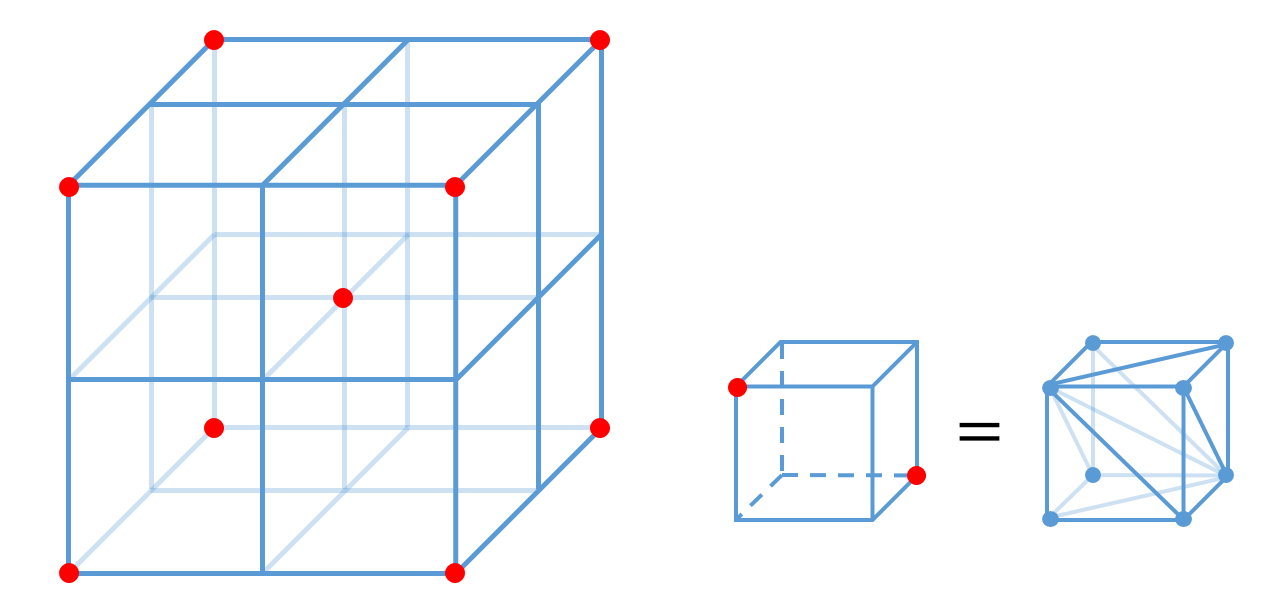
\includegraphics[width=0.45\textwidth]{images/holographic/3+1d-cube-2.png}}
  \caption[3+1 维中的三角剖分]{3+1 维中的三角剖分。(a) 每个正方体被分为了 6 个四面体。(b) 每个 $2\times2\times2$ 的大正方体包含了 8 个小正方体,三角剖分的方式由小正方体的对角(红色圆点)来决定。图片来源:\parencite{chen2022exact}。}
\end{figure}

如图~\ref{fig:rg-3+1d} 所示,3+1 维中的重整化大致通过以下三个步骤来实现:

\begin{enumerate}
  \item 消去边中间位置的顶点 $m$、$n$ 等,得到新的边 $\overline{12}$、$\overline{23}$ 等;
  \item 消去面中间位置的顶点 $\alpha$、$\beta$ 等,得到新的边 $\overline{13}$、$\overline{16}$ 等;
  \item 消去体心 $o$,得到新的边 $\overline{17}$。
\end{enumerate}

\begin{figure}[htb]
  \centering
  \subcaptionbox{重整化的总体效果}{%
    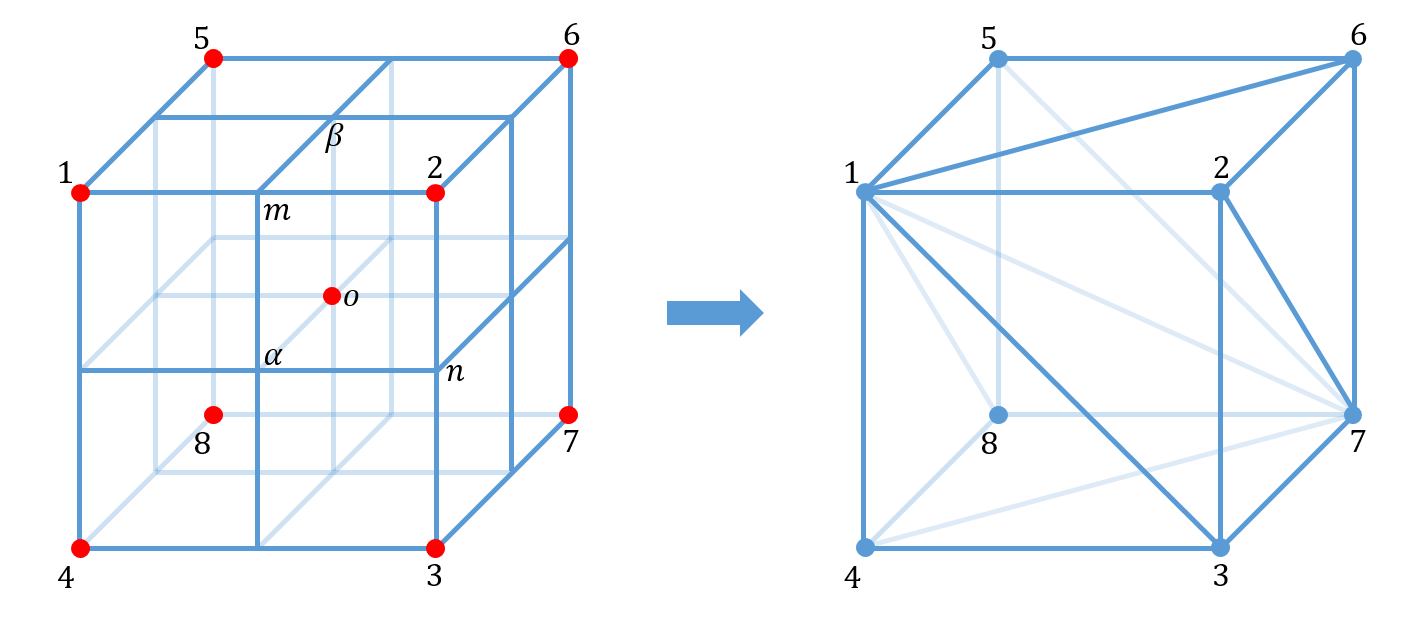
\includegraphics[width=0.45\textwidth]{images/holographic/rg-3+1d.png}} \quad
  \subcaptionbox{消去棱心 $m$,得到边 $\overline{12}$}{%
    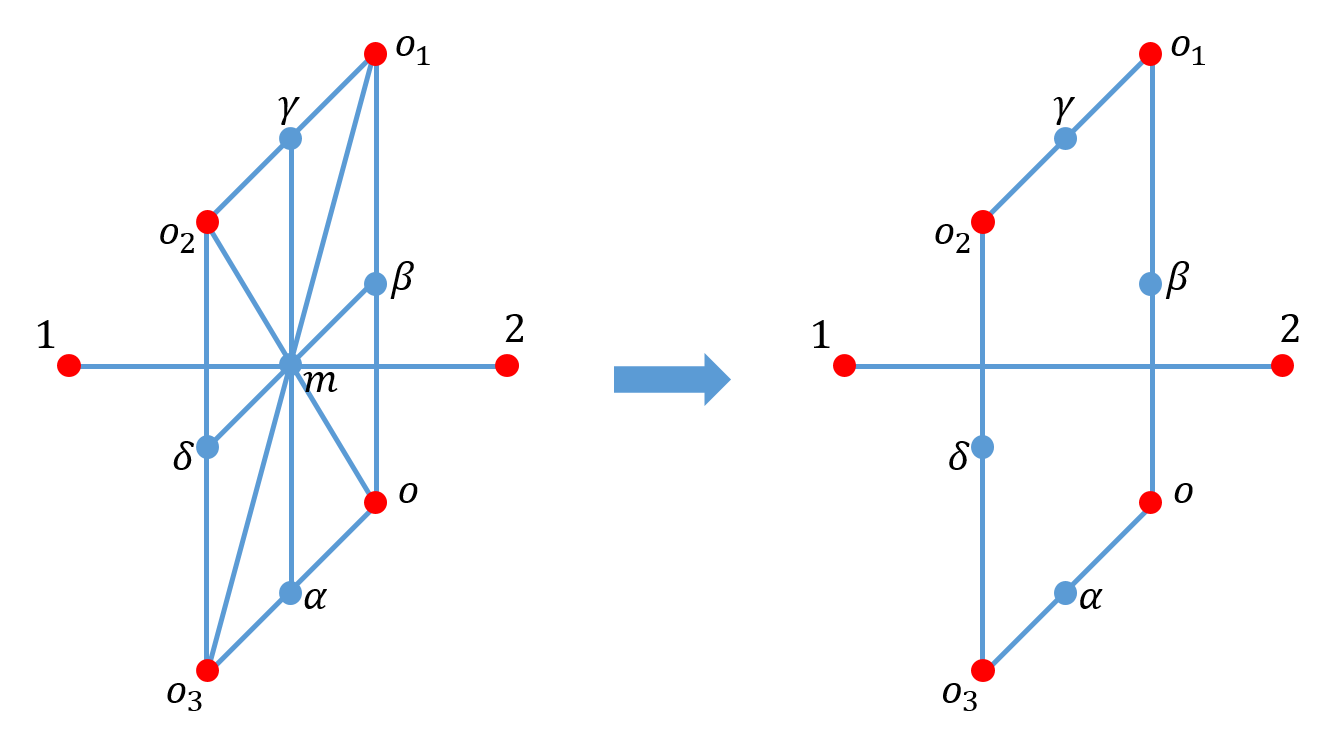
\includegraphics[width=0.45\textwidth]{images/holographic/rg-3+1d-step-1.png}} \\
  \subcaptionbox{消去面心 $\alpha$,得到边 $\overline{13}$}{%
    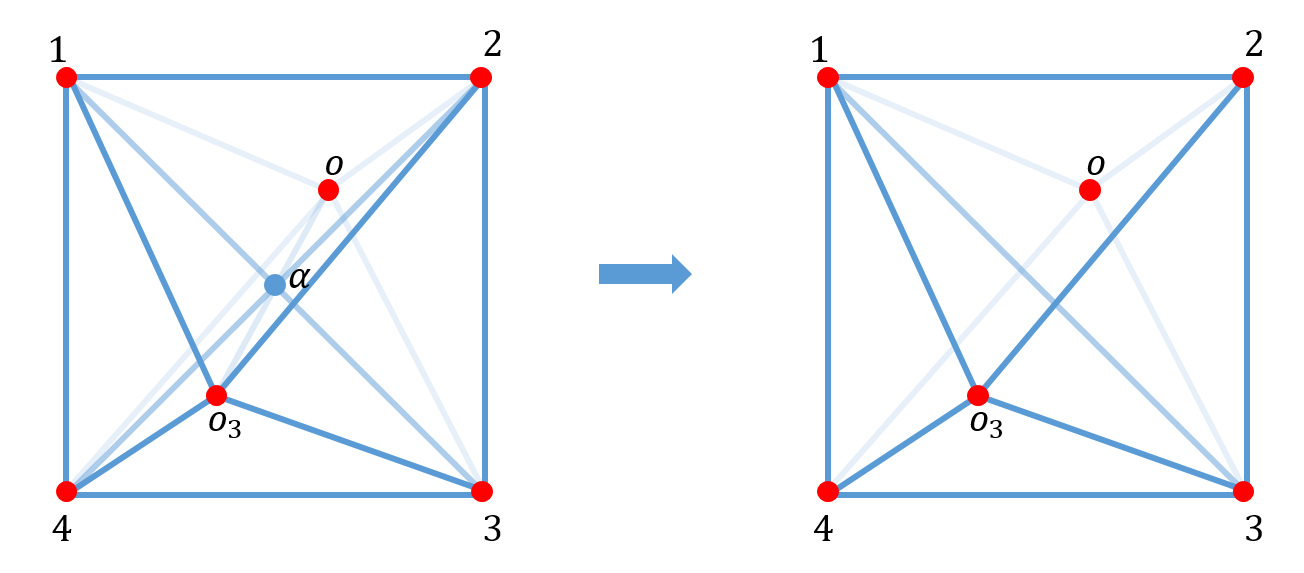
\includegraphics[width=0.45\textwidth]{images/holographic/rg-3+1d-step-2.png}} \quad
  \subcaptionbox{消去体心 $o$,得到边 $\overline{17}$}{%
    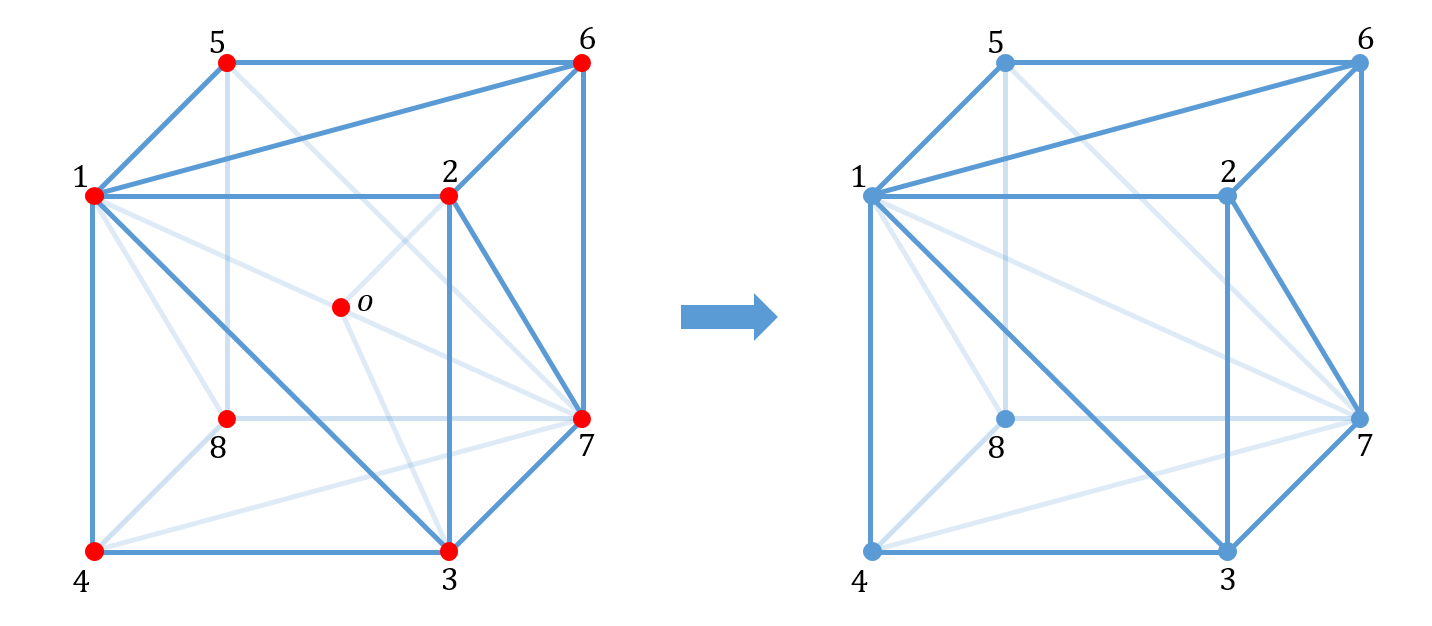
\includegraphics[width=0.45\textwidth]{images/holographic/rg-3+1d-step-3.png}}
  \caption[3+1 维中重整化算符的构造]{3+1 维中重整化算符的构造。$2\times2\times2$ 个正方体将被粗粒近似为 $1\times1\times1$ 个正方体。图片来源:\parencite{chen2022exact}。}
  \label{fig:rg-3+1d}
\end{figure}

考虑 3+1 维 toric code 模型(对应于 3+1 维 $\mathbb{Z}_2$ Dijkgraaf--Witten 模型)\cite{hamma2005string,zhao2022string},其边界态可以取为
\begin{equation}
  \bra{\Omega} = \sum_{\{a\}} \Omega_{\{a\}} \bra{\{a\}} = \bigotimes_e \bra{w_e},
\end{equation}
其中 $\bra{w_e}$ 是棱 $e$ 上的态。如图~\ref{fig:3+1d-cube-3} 所示,$\bra{w_e}$ 可分为两类:
\begin{equation}
  \bra{w_e} = \begin{cases}
    \bra{1} + \bra{-1}, & \text{red edges}; \\
    \ee^\beta \bra{1} + \ee^{-\beta} \bra{-1}, & \text{blue edges},
  \end{cases}
\end{equation}
由此得到的奇异关联子为
\begin{equation}
  Z = \langle\Omega|\Psi\rangle = \sum_{\{\sigma\}} \prod_{\ev{ij}} \ee^{\beta \sigma_i \sigma_j}
\end{equation}
可以发现它和三维 Ising 模型的配分函数是一致的。将正方体单元进一步拆分为四面体,可以给出 $\bra{\Omega}$ 的张量网络表示:
\begin{equation}
  \bra{\Omega(u_\beta)} = \sum_{\{a\}} \sum_{i,j,k,l,\dots} \cdots u_\beta^{ijkl} (a_1,a_2,a_3) \cdots \bra{\{a\}}.
\end{equation}
其中 $\sum_{\{a\}}$ 表示对所有可能的构型求和,而 $\sum_{i,j,k,l,\dots}$ 则表示对面上的指标求和,而张量单元
\begin{equation}
  u_\beta^{ijkl} (a,b,c) = \begin{cases}
    \ee^{\beta(a+2b+c)/8}, & i=j=k=l=1; \\
    0, & \text{otherwise}
  \end{cases}
\end{equation}
对应图~\ref{fig:3+1d-tetrahedron} 中的小四面体,其中 $a,b,c=\pm1$。

\begin{figure}[htb]
  \centering
  \subcaptionbox{\label{fig:3+1d-cube-3}}{%
    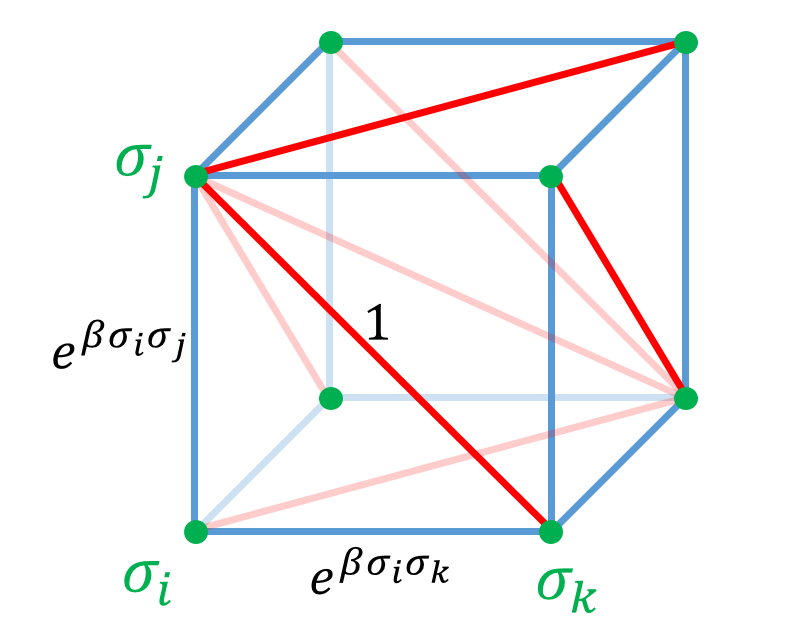
\includegraphics[width=0.3\textwidth]{images/holographic/3+1d-cube-3.png}} \qquad
  \subcaptionbox{\label{fig:3+1d-tetrahedron}}{%
    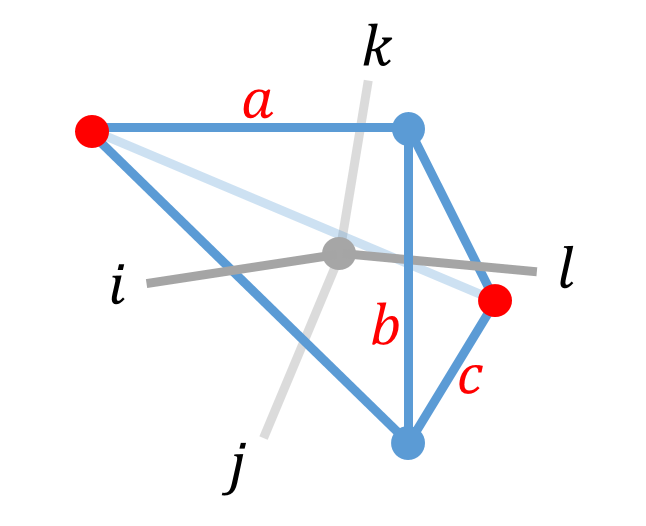
\includegraphics[width=0.25\textwidth]{images/holographic/3+1d-tetrahedron.png}}
  \caption[3+1 维 toric code 模型中的边界态]{3+1 维 toric code 模型中的边界态。(a) 边界中的棱分为红色和蓝色两类。(b) $a$、$b$、$c$ 表示棱上的自由度,$i$、$j$、$k$、$l$ 则是面上的指标。图片来源:\parencite{chen2022exact}。}
\end{figure}

按照上面介绍的重整化方案,我们可以找到 $u_\beta$ 的两个不动点,分别为 $u_0$ 和 $u_\infty$,而临界点大致为
\begin{equation}
  0.27 \lesssim \beta_{\text{c}} \lesssim 0.28,
\end{equation}
这与通过其他方法得到的三维 Ising 模型数值结果 $\beta_{\text{c}}=0.22165463(8)$\cite{hasenbusch2010finite}同样也是基本符合的(至一位有效数字)。注意到与 2+1 维的情况相同,这里连接维数仍然只取为 $\chi=1$。可以想见,增大连接维数将提高计算的精度。

\section{AdS/CFT 的张量网络重建}
\label{sec:ads-cft-tensor-network}

在上一节中,我们通过 $D+1$ 维拓扑格点模型构造了重整化算符,并且在 $D=1,2,3$ 的各维度中都给出了例子。将这些重整化算符不断堆叠,即取 $\lim_{N\to\infty}U(\mathcal{C})^N$,我们将得到一个类似 MERA 的张量网络结构(见 \ref{subsec:mps-generalization} 小节)。MERA 是一类全息张量网络,在给出特定的边界条件并使其能够流向不动点之后,它可以精确地描述 CFT。我们也通过三维 Ising 模型的例子展示了这一点。

此外,我们还注意到,奇异关联子的构造与 $p$-adic 张量网络也具有相似之处,而后者能够复现 $p$-adic AdS/CFT 中的诸多结论\cite{hung2019padic,chen2021emergent,chen2021bending1,chen2021bending2}。$p$-adic 张量网络的体态通过结合代数(CFT 算符的融合范畴)描述,而我们这里所采用的(高阶)融合范畴实际上是它的推广。在 $p$-adic 张量网络中,$p$-adic CFT 的配分函数也是以类似奇异关联子的形式给出的。在不动点处,边界态也对应了体全息张量网络的本征态。因此,我们这里的构造也有望用来实现 AdS/CFT 对应。

% \subsection{体—边传播子}

考虑在 \ref{subsec:holographic-tensor-network-2+1d} 小节中所探讨的二维 Ising 模型(即 $k=2$ 时的 $\mathcal{A}_{k+1}$ 模型)。我们在紫外 (UV) 层(图~\ref{fig:a-k+1-boundary-condition})和全息张量网络的第 $n$ 层分别插入两个算符,并数值地计算它们之间的关联函数,即
\begin{align}
     \ev[\big]{\mathcal{O}_{n=1}(x=y=0) \, \mathcal{O}_n(x,y)}
  &= \bigl\langle \Omega(T_{\Lambda_1}) \big|
     \sigma^z(x=y=0) \, U^{n-1}(\mathcal{C}) \, \sigma^z(x,y) \, U^n(\mathcal{C}) \cdots
     \big| \Psi \bigr\rangle \notag \\
  &= \bigl\langle \Omega(T_{\Lambda_1}) \big|
     \sigma^z(x=y=0) \, U^{n-1}(\mathcal{C}) \, \sigma^z(x,y)
     \big| \Psi_{\Lambda_n} \bigr\rangle.
\end{align}
计算结果如图~\ref{fig:bulk-boundary-propagator} 所示。可以发现,与上图相比,下图中对应于不同 $n$ 的点几乎都重叠在一起,这表明存在满足
\begin{equation}
  \ev{\mathcal{O}_1 \, \mathcal{O}_n} \sim \left[ \frac{z}{x^2+z^2} \right]^\Delta
\end{equation}
形式的\emph{体—边传播子} (bulk-boundary propagator)。这里所展示的只是一个初步结果,我们还需要对其他模型以及不同共形维数的算符进行进一步的检验。

\begin{figure}[htb]
  % TODO: update image
  \centering
  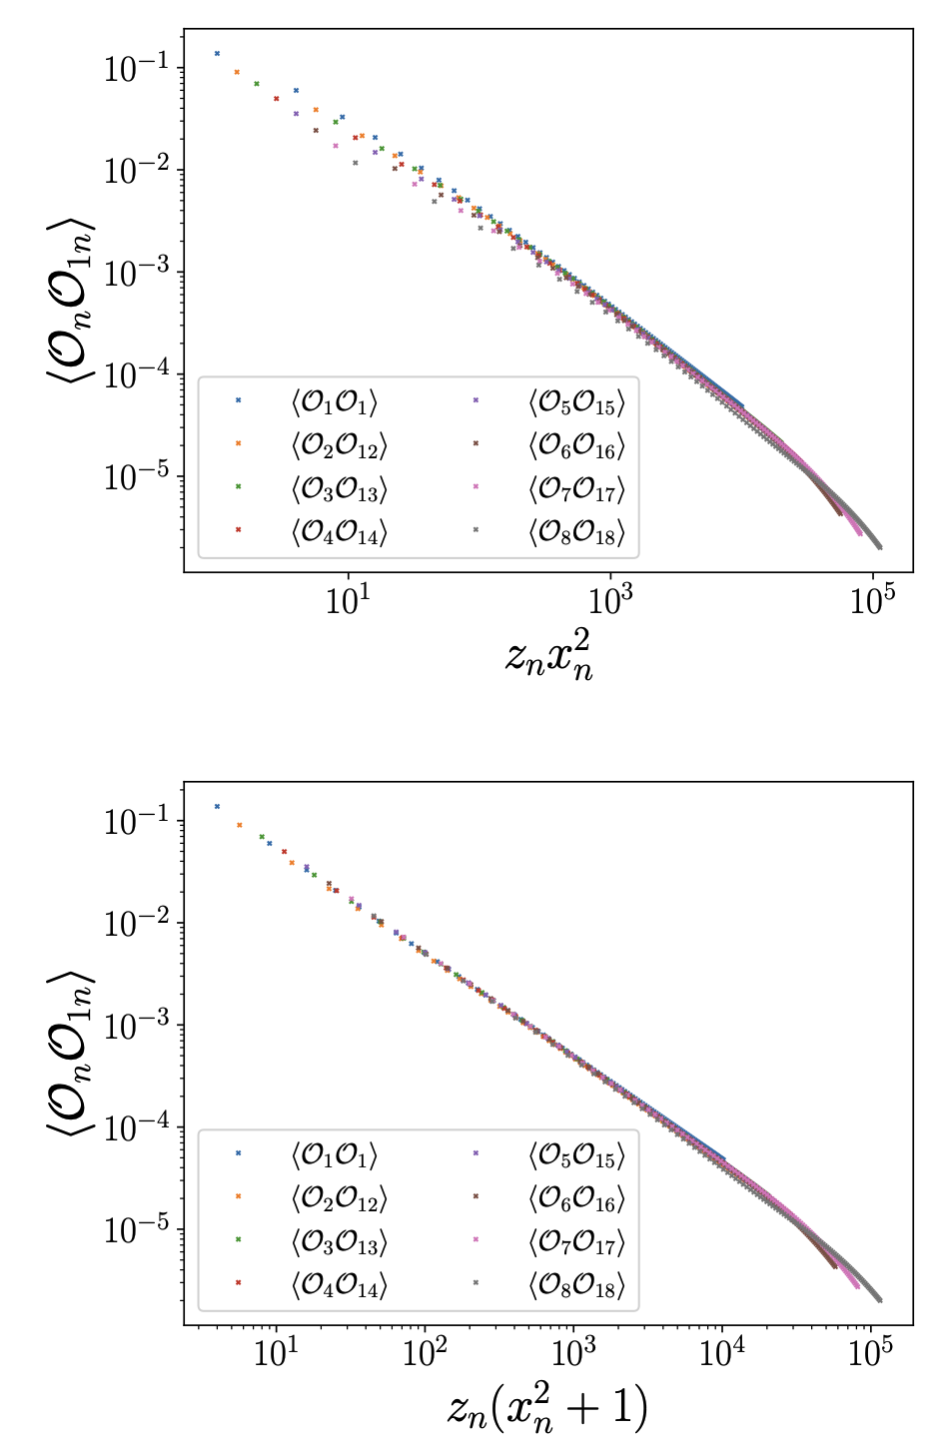
\includegraphics[width=0.5\textwidth]{images/holographic/bulk-boundary-propagator.png}
  \caption[体—边传播子的计算结果]{体—边传播子的计算结果。$\mathcal{O}_n$ 表示在第 $n$ 层插入的算符。为了计算方便,$\mathcal{O}_1$ 会和邻近的张量缩并,并推至第 $n$ 层,得到 $\mathcal{O}_{1n}$,因此 $\ev{\mathcal{O}_n\,\mathcal{O}_{1n}}$ 即相当于 $\ev{\mathcal{O}_n\,\mathcal{O}_1}$。(a)(b) 分别是关于 $z_n x_n^2$ 和 $z_n(x_n^2+1)$ 的 log-log 图像,其中 $z_n=(\sqrt{2})^{n-1}$,而 $x_n=x_1/z_n$ 是 $\mathcal{O}_n$ 和 $\mathcal{O}_{1n}$ 间的距离。在 AdS/CFT 字典中,有 $\ev{\mathcal{O}_n\,\mathcal{O}_1}\sim[z_n(x_n^2+1)]^{-\Delta}$,其中 $\Delta$ 是初级场 $\mathcal{O}_1$ 的共形维数。可以发现,在图 (b) 中对应于不同 $n$ 的点几乎都重叠在一起,这说明体—边传播子的形式是符合 AdS/CFT 预测的。图片来源:\parencite{chen2022exact}。}
  \label{fig:bulk-boundary-propagator}
\end{figure}

% TODO: entanglement wedge
% \subsection{Reconstruction Wedge}

\section{本章小结}

本章首先给出了弦网模型基态的 PEPS 张量网络表示,并通过将其与特定的直积态做内积得到奇异关联子。在 Fibonacci 和 Ising 两种模型中,我们利用奇异关联子构造了相应配分函数的张量单元,并通过 iTEBD 算法数值计算了对应 CFT 的中心荷。接下来,我们简要介绍了 PEPS 张量网络表示中的 MPO 对称性,而 MPO 所满足的推拉条件实质也是融合范畴中对称性的一种体现。我们还给出了管状代数与中心幂等元的构造,后者作为投影算符,可以给出 Drinfel'd 中心中不同的拓扑分区。最后,我们详细讨论了利用奇异关联子构建全息张量网络的方案。由于拓扑序的基态波函数 $\ket{\Psi}$ 位于重整化的不动点处,因而边界条件 $\ket{\Omega}$ 的选取就可以转化为重整化算符的本征值问题。我们在 1+1、2+1 和 3+1 维中分别给出了重整化算符及边界态的构造,并计算得到了临界点位置的初步数值结果。在二维 Ising 模型中,我们还利用全息张量网络计算了体—边传播子,并发现其形式与 AdS/CFT 的预测基本符合。
